\graphicspath{{Chapitre_4/Images/}}
\chapter{Thermodynamic components}\label{C4}
%%%%%%%%%%%%%%%%%%%%%%%%%%%%%%%%%%%
%%%%%                         %%%%%
%%%%% Introduction chapitre 3 %%%%%
%%%%%                         %%%%%
%%%%%%%%%%%%%%%%%%%%%%%%%%%%%%%%%%%
\quad\ In the beginning of the previous chapter, it has been mentioned that the Brayton cycle composed of several components that are more or less complex. The behavior of these components, which is required to realize the study of the global system, is based on the thermodynamic notions that have been introduced all along the past lines.

This chapter will be focused on the description of those components. For each of them, it will be provided the concepts or principles that will be used during this work. Then, a description of the Brayton cycle itself will be provided. Different configurations will be proposed and compared.
\section{Turbomachines}
%%%%%%%%%%%%%%%%%%%%%%%%%%%%%%%%%%%
%%%%%                         %%%%%
%%%%%    <<Turbomachines>>    %%%%%
%%%%%                         %%%%%
%%%%%%%%%%%%%%%%%%%%%%%%%%%%%%%%%%%
\quad\ The first family of components to be studied is the turbomachines. The machines included this family are ones ''that exchange energy between the
fluid traversing it and mechanical energy supplied to or extracted from the machine''\cite{Hillewaert2019}. Those machines are \textbf{rotating} machines
can be categorized into two families.

The first family of turbomachinery is ones which inject or extract energy from an incompressible flow. These transformations on the fluid  are respectively performed by pumps and hydraulic turbines.

The second family is turbomachines dealing with compressible flow. Here, some extra effects are taken into account. For instance, the velocity of the flow can be at some points limited due to choking effects. Also, since the flow is compressible its density can vary along the path, the velocity will vary along the path as well. These effects will be rediscussed in a future part of this section.

Turbomachines that are encompassed in this second category are compressors and gas turbines. As for the pumps and hydraulic turbines, compressors and turbines aim to inject and extract energy into/from the flow.

\subsection{General principles}
\quad\ Some principles used when designing incompressible and compressible flow based machines are common for both of these families. Among these principles, it can be emphasized the velocity triangle, the enthalpy and rhotalpy conservation, and the similarity analysis. The first ones provide tools to well design the blades of the turbomachinery, while the other principle is used to derive the performance of a given machine based on non-dimensional quantities. The following lines will explain the basis of these different principles. 

\subsubsection{Velocity triangle}
\quad\ When considering the rotating part of the turbomachine (named rotor), there is, in addition to the absolute frame of reference, a rotating frame which is attached to the rotor. This leads to definition of three components for the velocity of the fluid: 

\begin{itemize}
    \item Absolute velocity \(\mathbf{v}\): velocity of the fluid in the absolute frame (\(\mathbf{x},\mathbf{y}\)).
    \item Tip blade velocity of the rotor \(\mathbf{u_r}\): Velocity of the tip of the rotor blades in the absolute frame (\(\mathbf{x},\mathbf{y}\)).
    \item Relative velocity \(\mathbf{w_r}\): velocity of the fluid in the relative frame  (\(\mathbf{x'},\mathbf{y'}\)).
\end{itemize}

\begin{figure}[h]
    \centering
    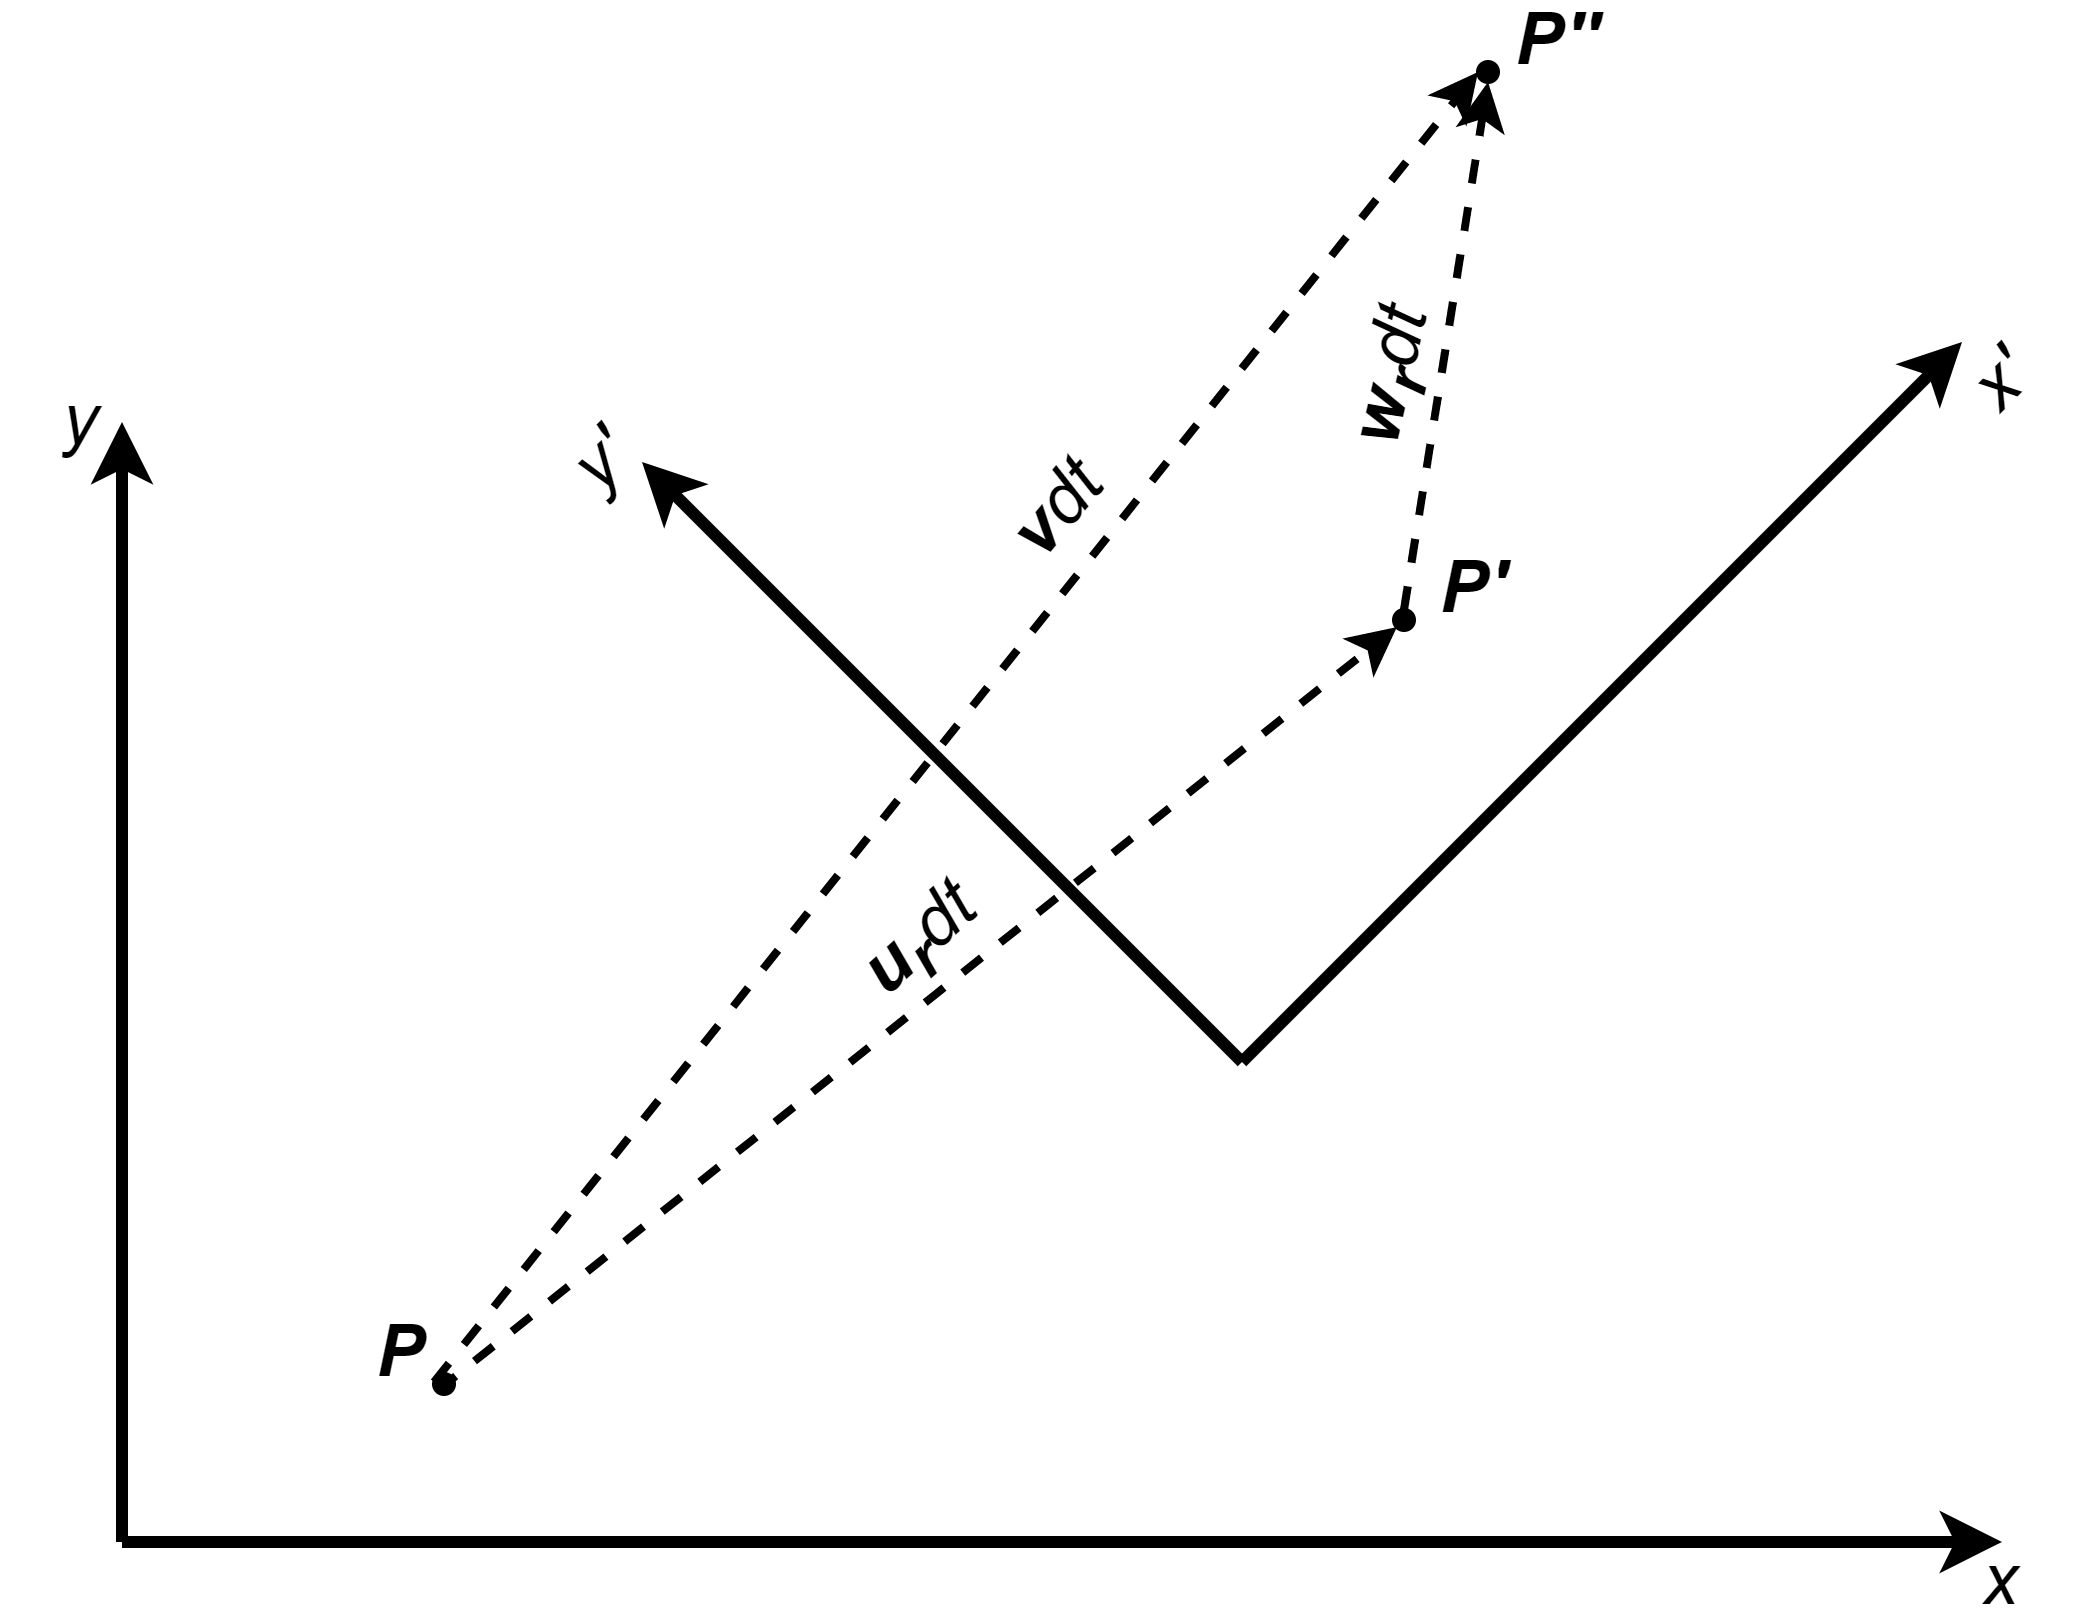
\includegraphics[width=0.6\textwidth]{Frames.png}
    \caption{Absolute and rotating frames.}
    \label{fig:C4_frames}
\end{figure}

The Figure \ref{fig:C4_frames} shows the representations in the space of these different definitions of the velocity. Considering a point at $P$ in the time t=0, this point is moving to \(P''\) in the time t=dt.  
The drawing shows that the following equality (\ref{eq:C4_velocity}) is enforced at any time.

\begin{equation}
    \setstretch{1}
    \mathbf{v} = \mathbf{u_r} + \mathbf{w_r} \label{eq:C4_velocity}
\end{equation}

Another way of representations of these velocities is to draw the velocity triangle. The velocity triangle is defined as depicted in the Figure \ref{fig:C4_vtriang}.

\begin{figure}[h]
    \centering
    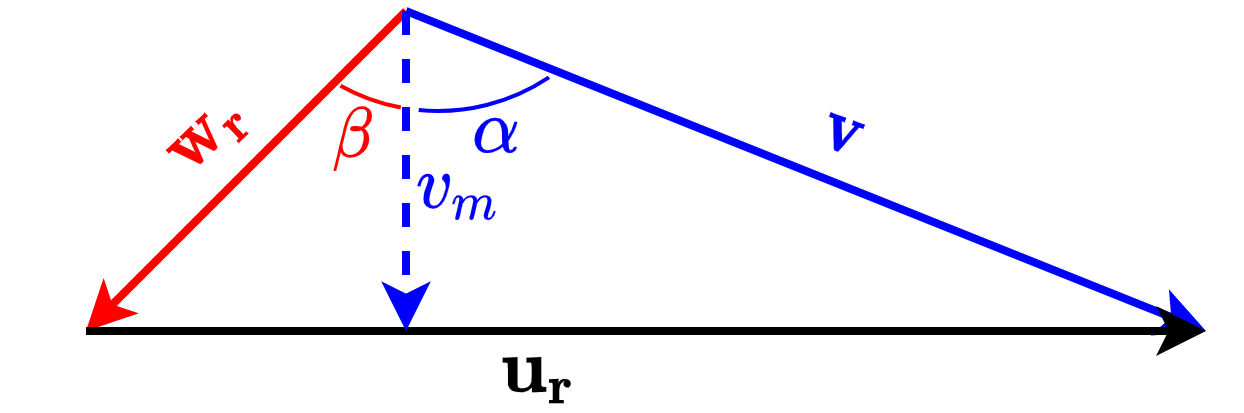
\includegraphics[width=0.6\textwidth]{Vtriangle.png}
    \caption{Velocity triangle.}
    \label{fig:C4_vtriang}
\end{figure}
Where $v_m$ is the projection of the vector $\mathbf{v}$ on the meridional axis.

Here, two angles $\alpha$ and $\beta$, respectively the absolute and relative flow angles, can be defined. Those angles will allow designing the shape of the rotating blade based on the desired applications. 

\subsubsection{Enthalpy and rothalpy conservation}
\quad\ It has been mentioned before that, for a compressible flow, the velocity can vary along the path. The notion of static and total (or stagnation) quantities have been established to take into account this variation of velocity. Stagnation quantities will be identified by the superscript ''0''.

For instance, the total enthalpy is given by
\begin{equation}
    \setstretch{1}
    h^0 = h + \frac{1}{2}\cdot v^2\label{eq:C4_h0}
\end{equation}

Now, considering an adiabatic transformation without viscous work, the total enthalpy is conserved between the initial state and the final state.
\begin{equation}
    \dot{m}_1\cdot h_1^0 = \dot{m}_2\cdot  h_2^0 \label{eq:C4_hcons}
\end{equation}
Which can be reduced to \(h_1^0 = h_2^0\) if we supposed that the transformation is performed without any leakages (\(\dot{m}_1=\dot{m}_2\)). The states \(1\) and \(2\) are associated to the orthogonal boundaries to the flow of the selected control volume delimiting the studied system.

\begin{equation}
    \setstretch{1}
    i^0 = h + \frac{1}{2}\cdot w_r^2 - \frac{1}{2}\cdot u_r^2 \label{eq:C4_i0}
\end{equation}

Similarly, using the definition (\ref{eq:C4_i0}) of the stagnation rhotalpy, it is obtained from the Euler equation (\ref{eq:C4_Euler}) that, within a rotor, the total rothalpy is conserved through the transformation process.

\begin{align}
    \setstretch{1}
    h_2^0 - h_1^0 = \frac{1}{2}\cdot & \left(v_2^2 - v_1^2\right) - \frac{1}{2}\cdot \left(w_{r,2}^2 - wr_{r,1}^2\right) + \frac{1}{2}\cdot \left(u_{r,2}^2 - u_{r,1}^2\right)\label{eq:C4_Euler} \\
    \text{with }                     & v = \left|\vect{v}\right|\quad\text{;}\quad  w_r = \left|\vect{w_r}\right|\quad\text{;}\quad u_r= \left|\vect{u_r}\right|\nonumber
\end{align}

The rhotalpy conservation is then expressed as stated in the equality (\ref{eq:C4_icons}).

\begin{equation}
    \setstretch{1}
    \dot{m}_1\cdot i_1^0 = \dot{m}_2\cdot i_2^0 \label{eq:C4_icons}
\end{equation} 

\subsubsection{Similarity}
\quad\ The design of the turbomachines often required validations through experimental testing.  

However, because the design of the turbomachines really depends on the application in view, creating a new test bench for each machine is time consuming and has a high cost. 

Thus, the analysis by similarity has been established to 
minimize the number of experimental campaign that has to be conducted. By defining some non-dimensional quantities describing the operating point of a given turbomachine, it is possible to extrapolate similar operating points of the same machine or, operating point of a similar machine of another size. 

This is a really powerful tool which allows to significantly decrease the time and the cost related to the design of a new turbomachines. Indeed, it allows to do the testing on smaller turbomachines, and then the performance of the desired machine are extrapolated. Since the machines and the associated test benches are smaller, the cost of the experimental campaign is significantly smaller, and the experimental results can be reused for future designed machines.

This concludes the introductory section about the basis notions to study the turbomachines. \newpage
\subsection{Pumps and hydraulic turbines}
\quad\, Now that the base principles have been introduced, those can be specified for the analysis of turbomachines performing transformation on incompressible flow. 

Among the machine exchanging energy with such type of fluid, it can be distinguish the pumps, which are designed to raise the height (or total hydraulic energy) \(h\) of the fluid, and the hydraulic turbines which do the opposite transformation. 

The variation of the height of the fluid is similar to its enthalpy variation. Thus, the respective power consumed and produced \(\dot{W}_p\) by  the pump and the hydraulic turbine can be expressed as given in relation (\ref{eq:C4_Pinc}), noting that the transformation makes the system going from state \textbf{a} to state \textbf{b}.
\begin{equation}
    \dot{W}_{p,a-b} = \dot{m}\cdot (h_a - h_b)=\dot{m}\cdot\Delta h_p \label{eq:C4_Pinc}
\end{equation}


If the consumed power of the pump is \(\dot{W}_{e,a-b}\), its global efficiency \(\eta_p\) is equal to the ratio
\begin{equation}
    \eta_p = \frac{\dot{W}_{p,a-b}}{\dot{W}_{e,a-b}}\label{eq:C4_Etapump}
\end{equation}
\subsubsection{Characteristic maps}
\quad\ It has been shown that the power output and the global efficiency of the pump are functions of the height variation and the flow rate of the fluid. When operating a pump, it can be useful to know how this height variation will vary with respect to the flow rate and the rotational speed of the pump shaft. The knowledge of these two parameters allows to fully characterized the pump.

Considering the volumetric flow rate \(\dot{\mathrm{V}}\) (m$^3$/s) and the rotational speed \(N\), the two following relations (\ref{eq:C4_DHp}) and (\ref{eq:C4_Pe}) can be derived.

\begin{subequations}
    \setstretch{1}
    \begin{equation}
        \Delta h_p(\dot{\mathrm{V}}_p, N_p)\label{eq:C4_DHp}\\
    \end{equation}
    \begin{equation}
        \dot{W}_{elec}(\dot{\mathrm{V}}_p, N_p)\label{eq:C4_Pe}
    \end{equation}
\end{subequations}
Those relations will be called characteristic or performance map and has to be determined \textbf{experimentally}. An example of such map is given in the Figure \ref{fig:C4_MapPump}.
\begin{figure}[h]
    \centering
    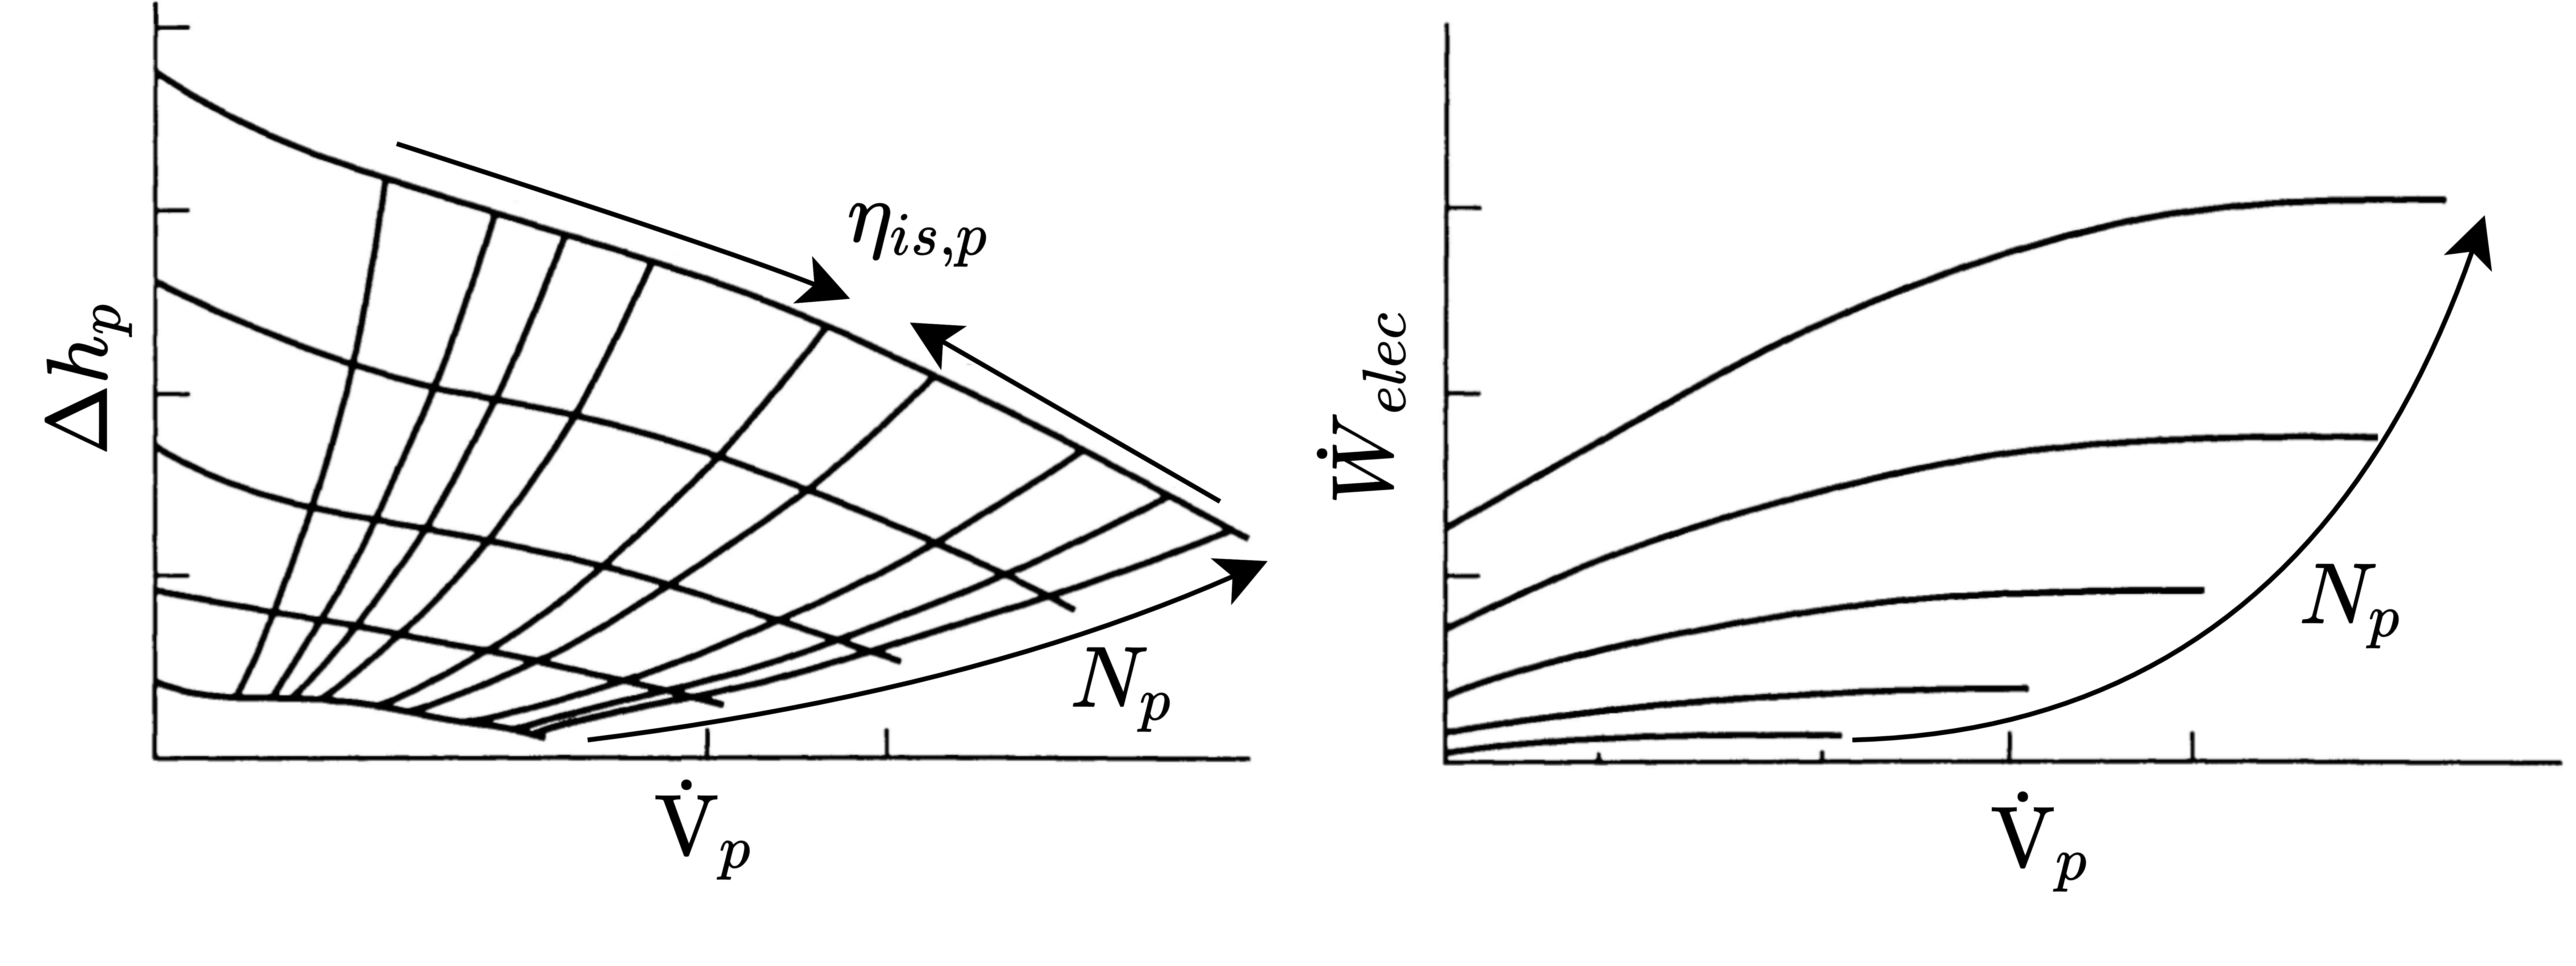
\includegraphics[width=0.8\textwidth]{Pump_map.png}
    \caption{Characteristic maps of a pump \cite{Hillewaert2019}.}
    \label{fig:C4_MapPump}
\end{figure}

However, not all the operating points constituting the performance map has to be computed through an experimental campaign. Indeed, using the similarity analysis described during the previous section, determining the operating points for one rotational speed is sufficient to deduce the rest of the characteristic map.

\begin{subequations}
    \begin{equation}
        \phi = \frac{\dot{\mathrm{V}_p}}{N_p\cdot r_2^3}\label{eq:C4_phipump}
    \end{equation}
    \begin{equation}
        \psi = \frac{4\cdot g\cdot \Delta h_p}{N_p^2\cdot r_2^2}\label{eq:C4_psipump}
    \end{equation}
\end{subequations}

For the pump, the head and flow non-dimensional coefficients \(\phi\) and \(\psi\) are defined based on the outlet condition \textbf{2} of the pump. Those coefficients are respectively defined by the relations (\ref{eq:C4_phipump}) and (\ref{eq:C4_psipump}), \(r_2\) being the outlet radius of the pump. 

From the definitions of these two non-dimensional quantities, the height variation \(\Delta h_p\) and the volumetric flow rate $\dot{\mathrm{V}}$ can be obtained for any rotational speed. 

Considering that the operating point (\(\dot{\mathrm{V}}_1, \Delta h_{p,1},N_1\)) is known, the similar operating point\linebreak (\(\dot{\mathrm{V}}_2, \Delta h_{p,2},N_2\)) for any rotational speed \(N_2\) can be obtained using the relations (\ref{eq:C4_Qsim}) and (\ref{eq:C4_DHsim}).

\begin{subequations}
    \setstretch{1}
    \begin{equation}
        \dot{\mathrm{V}}_{p,2} = \dot{\mathrm{V}}_{p,1}\cdot\frac{N_{p,2}}{N_{p,1}} \label{eq:C4_Qsim}
    \end{equation}
    \begin{equation}
        \Delta h_{p,2} = \Delta h_{p,1}\cdot\left(\frac{N_{p,2}}{N_{p,1}}\right)^2 \label{eq:C4_DHsim}
    \end{equation}\label{eq:C4_sim}
\end{subequations}

These relations stand since for any similar point of operation, the non-dimensional quantities remain constant. Consequently, the pump isentropic efficiency remains constant as well.

Similar reasoning can be performed for the hydraulic turbines. For hydraulic turbines, the head and flow coefficients are defined based on the inlet condition \textbf{1} of the turbines.

\subsection{Compressible flow}
\quad\ The previous subsection introduced the pump which is a turbomachine design to increase the energy of the incompressible fluid passing through it. However, this type of machine cannot deal with compressible flow for which the density can vary over the distance. For instance, the air is a compressible fluid.

The behavior of the compressible flow is more complex to describe compared to incompressible flow. Indeed, “compressible flow is characterized by the propagation of acoustic waves” \cite{Hillewaert2019}.   This part of the section about turbomachines will only focus on the main principles required for the good understanding of this work.


\subsubsection{Velocity triangle}
\quad\ With the relation (\ref{eq:C4_Euler}), the notion of absolute and relative velocity of the flow has been introduced. A graphic representation of these three vectors can be done using the \textbf{velocity triangle}. This triangle is drawn in the Figure \ref{fig:C4_vtriang}.

\subsubsection{Mach number}
The Mach number \(M\) is defined as being the ratio between the velocity \(v\) and the sound speed \(c\).
\begin{equation}
    M = \frac{v}{c} \label{eq:C4_Mach}
\end{equation}
The Mach number \(M\) is a dimensionless variable that gives an image of the compressible effects of the flow. Thus, one criterion for the determination of similar operational points is to keep the Mach number constant.

Using the Mach number allows obtaining formulas to compute the total quantities based on the static ones. By considering first the total temperature, the relation (\ref{eq:C4_TT0_1}) can be found.
\begin{equation}
    T^0 = T + \frac{v^2}{2\cdot c_p} = T\cdot\left(1 + \frac{v^2}{2\cdot c_p\cdot T}\right)\label{eq:C4_TT0_1}
\end{equation}
For an isentropic process, it can be demonstrated that the speed of sound \(a=k\cdot r\cdot T\). Thus, the equation (\ref{eq:C4_TT0_1}) becomes (\ref{eq:C4_TT0})
\begin{equation}
    T^0 = T\cdot\left(1 + \frac{k-1}{2}\cdot M^2\right) = T\cdot f_M(M) \label{eq:C4_TT0}
\end{equation}
Using the equations (\ref{eq:C3_isrelPT}), (\ref{eq:C3_isrelrhoT}) from chapter \ref{C3} and the definition of the function \(f_M(M)\), the relations linking the static to the total pressure, density and speed of sound can be obtained as well.

\begin{subequations}
    \setstretch{1}
    \begin{equation}
        p^0 = p\cdot f_M(M)^\frac{k}{k-1}\label{eq:C4_PP0}
    \end{equation}
    \begin{equation}
        \rho^0 = \rho\cdot f_M(M)^\frac{1}{k-1}\label{eq:C4_rhorho0}
    \end{equation}
    \begin{equation}
        c^0 = c\cdot\sqrt{f_M(M)} \label{eq:C4_aa0}
    \end{equation}
\end{subequations}

\subsubsection{Characteristic maps}
\quad\ As for the turbomachines exchanging energy with incompressible flow, those dealing with compressible flow can also be fully characterized knowing a pair of independent operating parameters. The most usual parameters are

\begin{itemize}
    \setstretch{1}
    \item \(\dot{m}_{corr}\) (kg/s): It is the corrected mass flow rate.
    \item \(\Pi_{tt}\) (-): It is the total to total pressure ratio between the inlet and the outlet of the turbomachine. If the turbomachine is compressing the flow, the ratio is reverse to keep it greater than one.
    \item \(N_{corr}\) (RPM): It is the corrected rotational speed of the turbomachine. 
    \item \(\eta_{is}\) (-): It is the total to total isentropic efficiency of the turbomachine.
\end{itemize}
It can be demonstrated that the performance map of a turbomachine is ''determined by the relation between 3 non-dimensional groups.''\cite{Hillewaert2019}. 

Considering an operating point $a$ characterized by the mass flow rate $\dot{m}_a$, the rotational speed $N_a$, and the inlet stagnation temperature and pressure $T^0_{1,a}$ and $p^0_{1,a}$, it is possible to derive any similar operating points. By applying the formula (\ref{eq:C4_mab}) and (\ref{eq:C4_Nab}), the mass flow rate $\dot{m}_b$ and rotational speed $N_b$ at the similar operating point $b$ characterized by the stagnation inlet state ($T^0_{1,b}$, $p^0_{1,b}$) can be computed.
\begin{subequations}
\begin{align}
\setstretch{1}
    \dot{m}_{b} &= \dot{m}_{a}\cdot\sqrt{\frac{T^0_{1,a}}{T^0_{1,b}}}\cdot\frac{p^0_{1,b}}{p^0_{1,a}}\label{eq:C4_mab}\\
    N_b &= N_a\cdot \sqrt{\frac{T^0_{1,b}}{T^0_{1,a}}}\label{eq:C4_Nab}
\end{align}    
\end{subequations}

These two relations allow to goes from one operating point to the other without modifying the value of the non-dimensional quantities. Therefore, going from $a$ to $b$ will not modify the pressure ratio $\Pi_{tt}$, the isentropic efficiency $\eta_{is}$ and the Mach number $M$.

In particular, if the operating point $b$ considered is defined at the reference conditions ($T_{ref},P_{ref}$), the associated mass flow rate and rotational speed are called \textbf{corrected} mass flow rate $\dot{m}_{corr}$ and \textbf{corrected} rotational speed $N_{corr}$. Thus, from a measured operating point, these two corrected quantities are obtained by applying the relation (\ref{eq:C4_mc}) and (\ref{eq:C4_Nc}).

\begin{subequations}
\setstretch{1}
\begin{align}
    \dot{m}_{corr} &= \dot{m}\cdot \frac{\sqrt{\theta_T}}{\theta_p}\label{eq:C4_mc}\\
    N_{corr} &= \frac{N}{\sqrt{\theta_T}}\label{eq:C4_Nc}
\end{align}    
\end{subequations}
Where $\theta_T = \frac{T^0}{T_{ref}}$ and $\theta_p = \frac{p^0}{p_{ref}}$. $T^0$ and $p^0$ are respectively the stagnation temperature and pressure observed at the inlet of the turbomachine.

Alternatively, the reduced mass flow rate \(\dot{m}_{r}\) can also be used to assess the performance of the turbomachines. This non-dimensional quantity is as follows:

\begin{equation}
    \setstretch{1}
    \dot{m}_r = \dot{m}\cdot \frac{\sqrt{T^0}}{p^0}
\end{equation}

Now, if the rotational speed $N$ and the mass flow rate $\dot{m}$ are assumed to be known, the two other quantities ($\Pi_{tt}$) and ($\eta_{is}$) can be calculated using the relations (\ref{eq:C4_Pimap}) and (\ref{eq:C4_etamap}).

\begin{subequations}
    \setstretch{1}
    \begin{equation}
        \Pi_{tt}(N_{corr}, \dot{m}_{corr})\label{eq:C4_Pimap}
    \end{equation}
    \begin{equation}
        \eta_{is}(N_{corr}, \dot{m}_{corr})\label{eq:C4_etamap}
    \end{equation}
\end{subequations}
These relations can be established by the means of experimental measurements.
\subsection{Gas compressor}
\quad\ The previous lines show some properties of compressible flows that add complexity to the analysis. Now, it is interesting to describe two types of turbomachines inducing a modification of the state of the flow.

The first category of machines to be considered is the compressor. As for the pumps, the compressor can be axial or centrifugal.  The axial compressor is mainly composed of a rotating part (the rotor), followed by a non-moving part (the stator) converting the kinetic energy at the exit of the rotor into pressure. A diagram of an axial compressor stage is given in the Figure \ref{fig:C4_compstage}.

\begin{figure}[h]
    \centering
    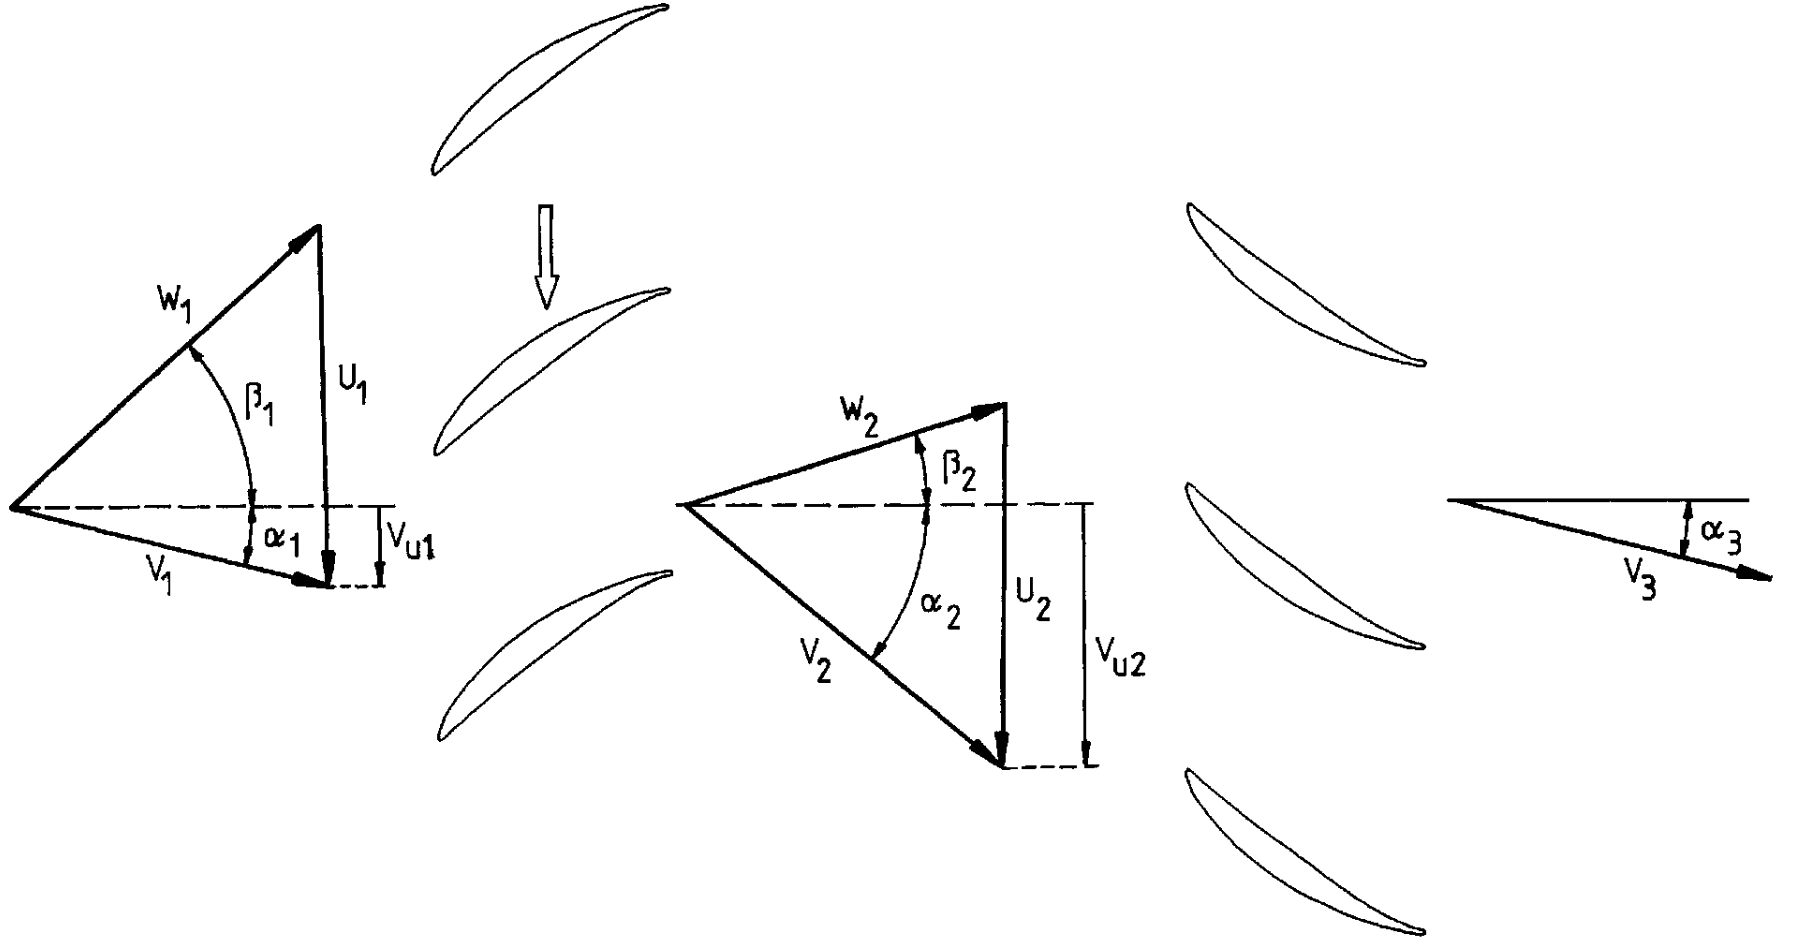
\includegraphics[width=0.5\textwidth]{Comp_stage.png}
    \caption{Axial compressor stage \cite{Hillewaert2019}.}
    \label{fig:C4_compstage}
\end{figure}

The entities between each velocity triangles are the blades of the rotor (emphasized by an arrow) or of the stator. It can be observed that the rotor blades increase the value of the flow velocity \(v\). As explained earlier this augmentation of kinetic energy is then recovered by the stator blades.

\subsubsection{Mollier diagram}
\quad\ The transformation induced by the compressor can be represented into a h-s diagram also named the Mollier diagram. The Mollier diagram for one compressor stage has been drawn in the Figure \ref{fig:C4_Molliercomp}.

\begin{figure}[h]
    \centering
    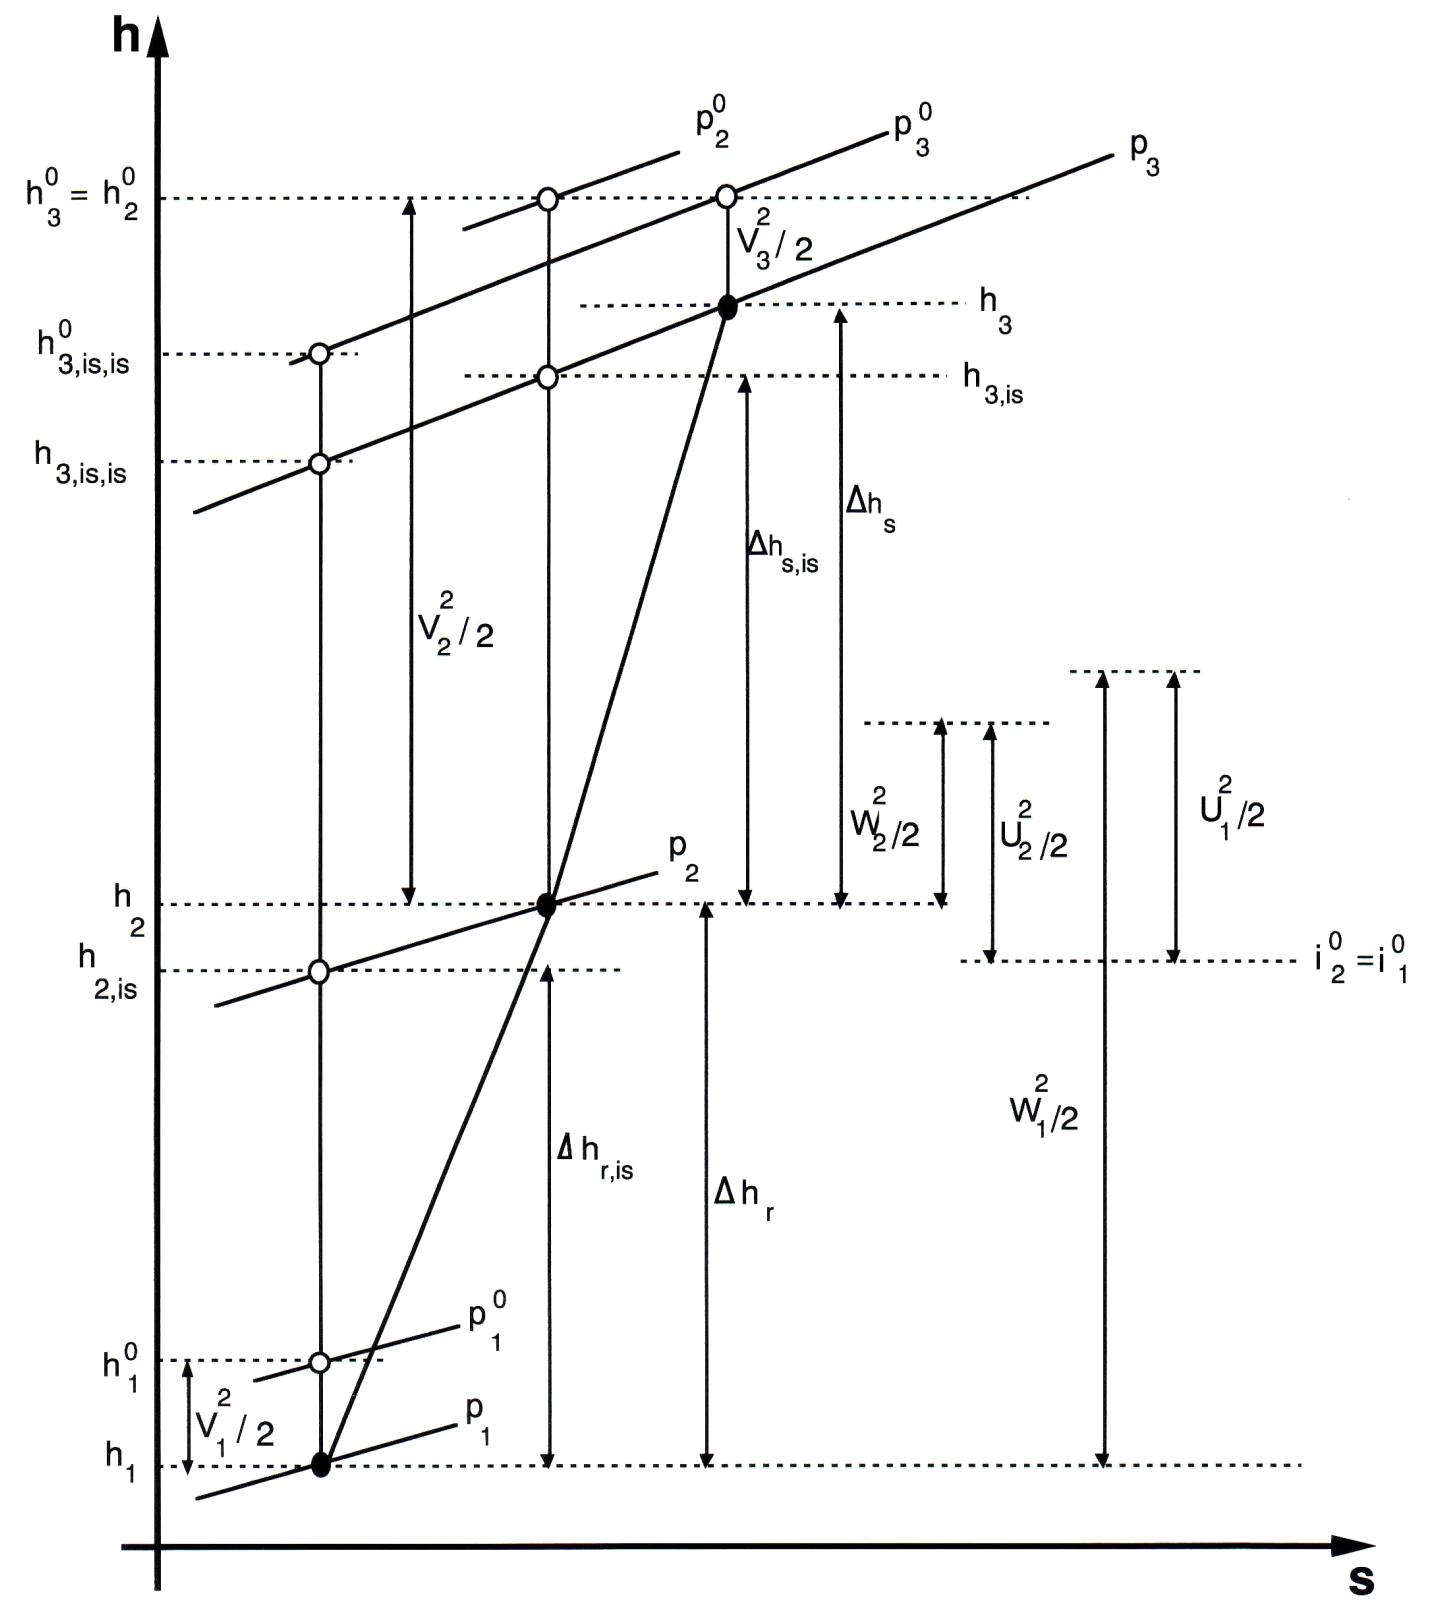
\includegraphics[width=0.5\textwidth]{Comp_mollier.png}
    \caption{Mollier diagram of a compressor stage \cite{Hillewaert2019}}
    \label{fig:C4_Molliercomp}
\end{figure}

The diagram, for which the velocity triangles are given in the Figure \ref{fig:C4_compstage}, has to be read as follows.
\begin{itemize}
    \setstretch{1}
    \item State \textbf{1}: Starting from the static enthalpy and pressure \(h_1\) and \(p_1\), the relations (\ref{eq:C4_i0}), (\ref{eq:C4_h0}) and (\ref{eq:C4_PP0}) are used to calculate the total enthalpy, rothalpy and pressure.
    \item State \textbf{2}: The transformation \textbf{1}-\textbf{2} takes place within the rotor of the compressor stage. Thus, the total rothalpy is conserved over the transformation ($i_2^0=i_1^0$).

    The knowledge of the total rothalpy allows determining the other quantities. The static enthalpy (and by extension the total enthalpy) can be deduced using the relation (\ref{eq:C4_i0}). Concerning the pressure, there is an increase of the static and total pressure of the fluid “due to the diffusion in the rotor passage” \cite{Hillewaert2019} ($p_2^{(0)} > p_1^{(0)}$).

    \item State \textbf{3}: The transformation \textbf{2}-\textbf{3} takes place within the stator of the compressor stage. Thus, the total enthalpy is conserved over the transformation ($h_3^0 = h_2^0$).

    Then, the static enthalpy can be computed using the relation (\ref{eq:C4_h0}). The conversion of the kinetic energy into pressure leads to an increase of the static and total pressure ($p_3^{(0)} > p_2^{(0)}$).
\end{itemize}
As a reminder, the enthalpy at the end of the process is higher than the one considering an isentropic transformation.
\subsubsection{Performance maps}
\quad\ As for any turbomachines, the compressor can be characterized by its performance map. The map is composed of the performance plot often completed with the efficiency hill. The performance plot provides the total to total pressure ratio \(\Pi_{tt,c}\) as a function of the corrected rotational speed \(N\) and mass flow rate \(\dot{m}_c\).

An illustration of a compressor performance map is given in the Figure \ref{fig:C4_compmap}.
\begin{figure}[h]
    \centering
    \includegraphics[width=0.6\textwidth]{Comp_Map.png}
    \caption{Illustration of a compressor performance map \cite{Dixon2013}.}
    \label{fig:C4_compmap}
\end{figure}

Three types of curve are emphasized on the graph. The solid line are each associated to one set of operating point characterized by the same corrected rotational speed $N_{corr,c}$. It can be noticed that each iso-rotational speed curve goes asymptotically to the infinity at a given corrected mass flow rate. This value corresponds to the maximal mass flow rate that can goes through the compressor and is associated to the phenomenon called choking. 

This maximal mass flow rate $\dot{m}_{choke,c}$ is strongly dependent of the stagnation conditions of the flow. It can be shown that the value of the mass flow rate is proportional to the stagnation pressure and inversely proportional to the square root of the stagnation temperature.
Increasing the rotational speed of the compressor has the effect to increase these stagnation quantities. Since the total pressure increases faster than the total temperature, the maximal flow rate due to the choking will increase with the rotational speed.

Then, there are the doted lines represent the isentropic efficiency contours. These contours produce together what will be called the efficiency hill.

Finally, the red doted line is called instability line or surge line. The surge line provides a lower bound for the mass flow rate going through the compressor. At this minimal flow rate, the flow starts to stall in the machine. Going beyond this limit would lead to a backward flow in the compressor, causing irreversible damages to the compressor. Thus when operating the machine, a certain margin is taken with respect to the surge line.

In the Figure \ref{fig:C4_compmap},  the iso-rotational speed curves start from 70\% of the nominal rotational speed to a 102,5\%. This implies that the map is not defined for the operating points characterized by a low rotational speed. This is generally the case for most of the compressor maps. However, for the low rotational speeds, the flow can be supposed incompressible. Using this approximation, it is possible to use the rules of similarity described in the section about pumps to extrapolate the map to the lower rotational speeds.

\subsection{Gas turbine}
\quad\ From now, only compressor has been introduced. However, in a gas cycle, the compressor is combined with a turbine that will expand the gas. Only for some exception, the turbine is always placed after the combustion chamber. This choice allows providing to the turbine a flow with very high enthalpy.

Typically, an axial gas turbine is composed of a stator followed by a rotor. The stator is designed to create a deflection of the flow in the sense of rotation of the rotor. This will accelerate the flow before entering the rotor.

The schematic of an axial turbine stage is drawn in the Figure \ref{fig:C4_turbstage}.
\begin{figure}[h]
    \centering
    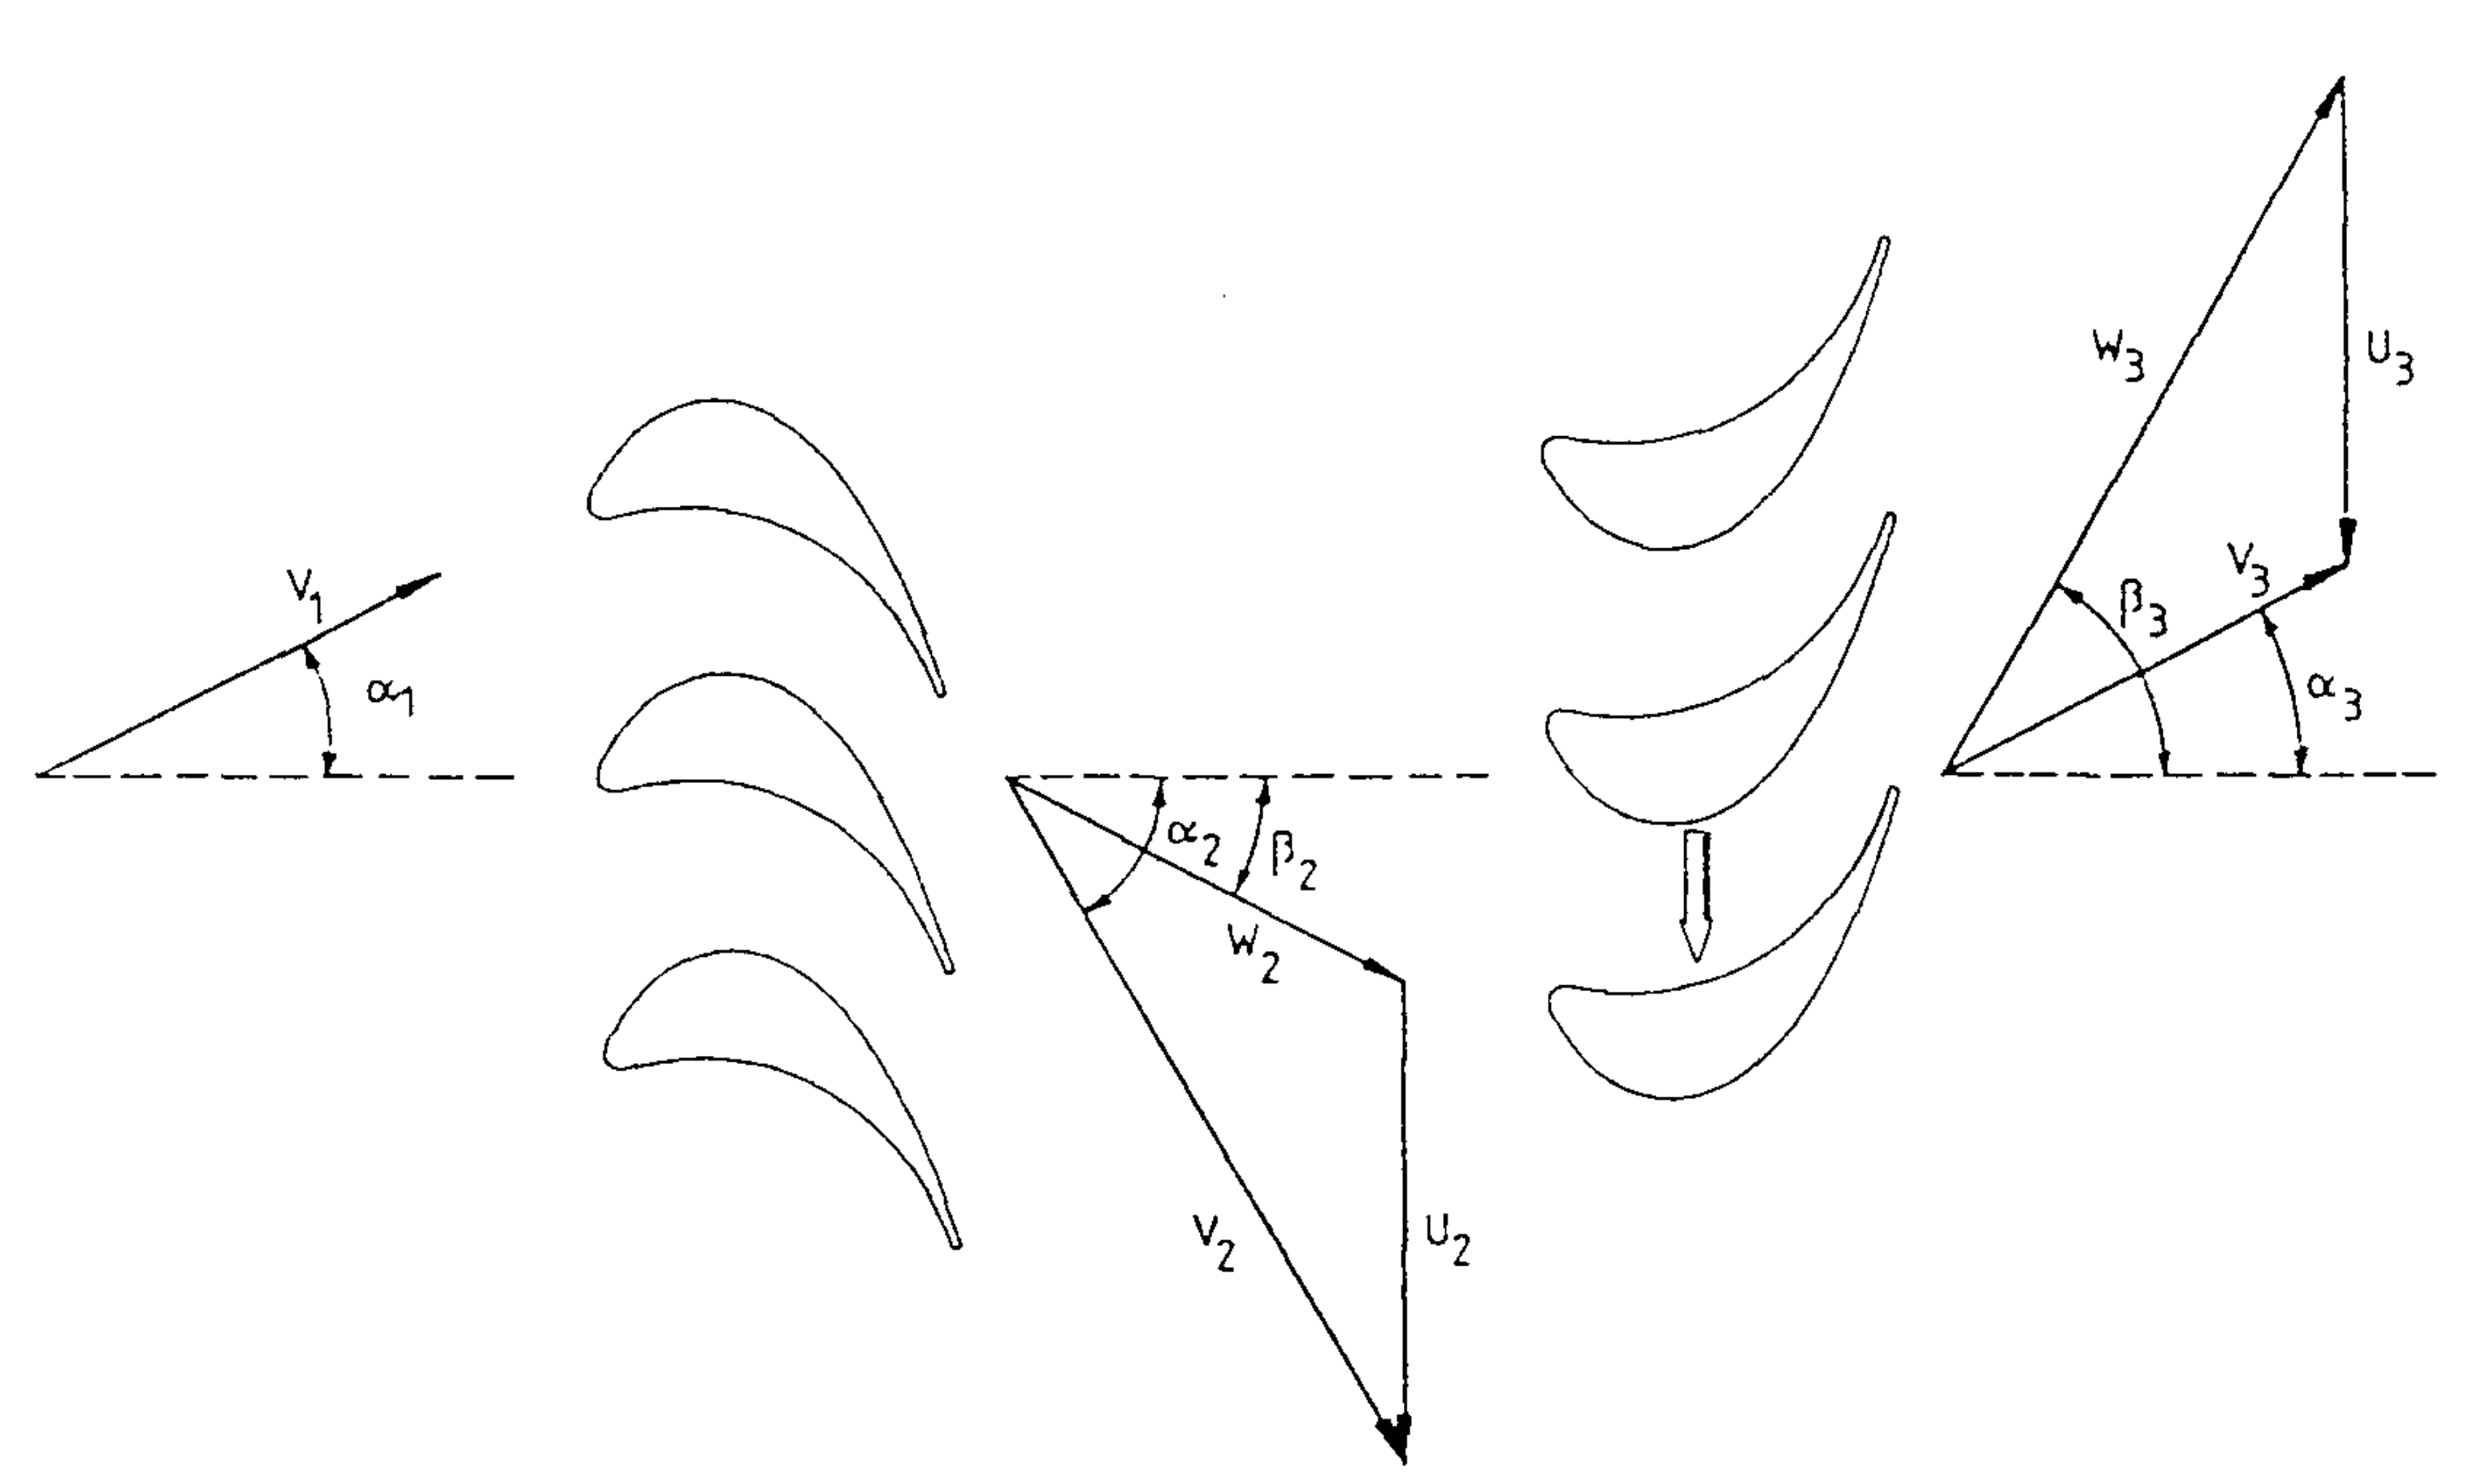
\includegraphics[width=0.5\textwidth]{Turb_stage.png}
    \caption{Axial turbine stage \cite{Hillewaert2019}.}
    \label{fig:C4_turbstage}
\end{figure}
\subsubsection{Mollier diagram}
As for the compressor, the real expansion induced by the turbine can be represented into a Mollier diagram. The diagram is depicted in the Figure \ref{fig:C4_Mollierturb}. The methodology to read the diagram is the same as before.

\begin{figure}[h]
    \centering
    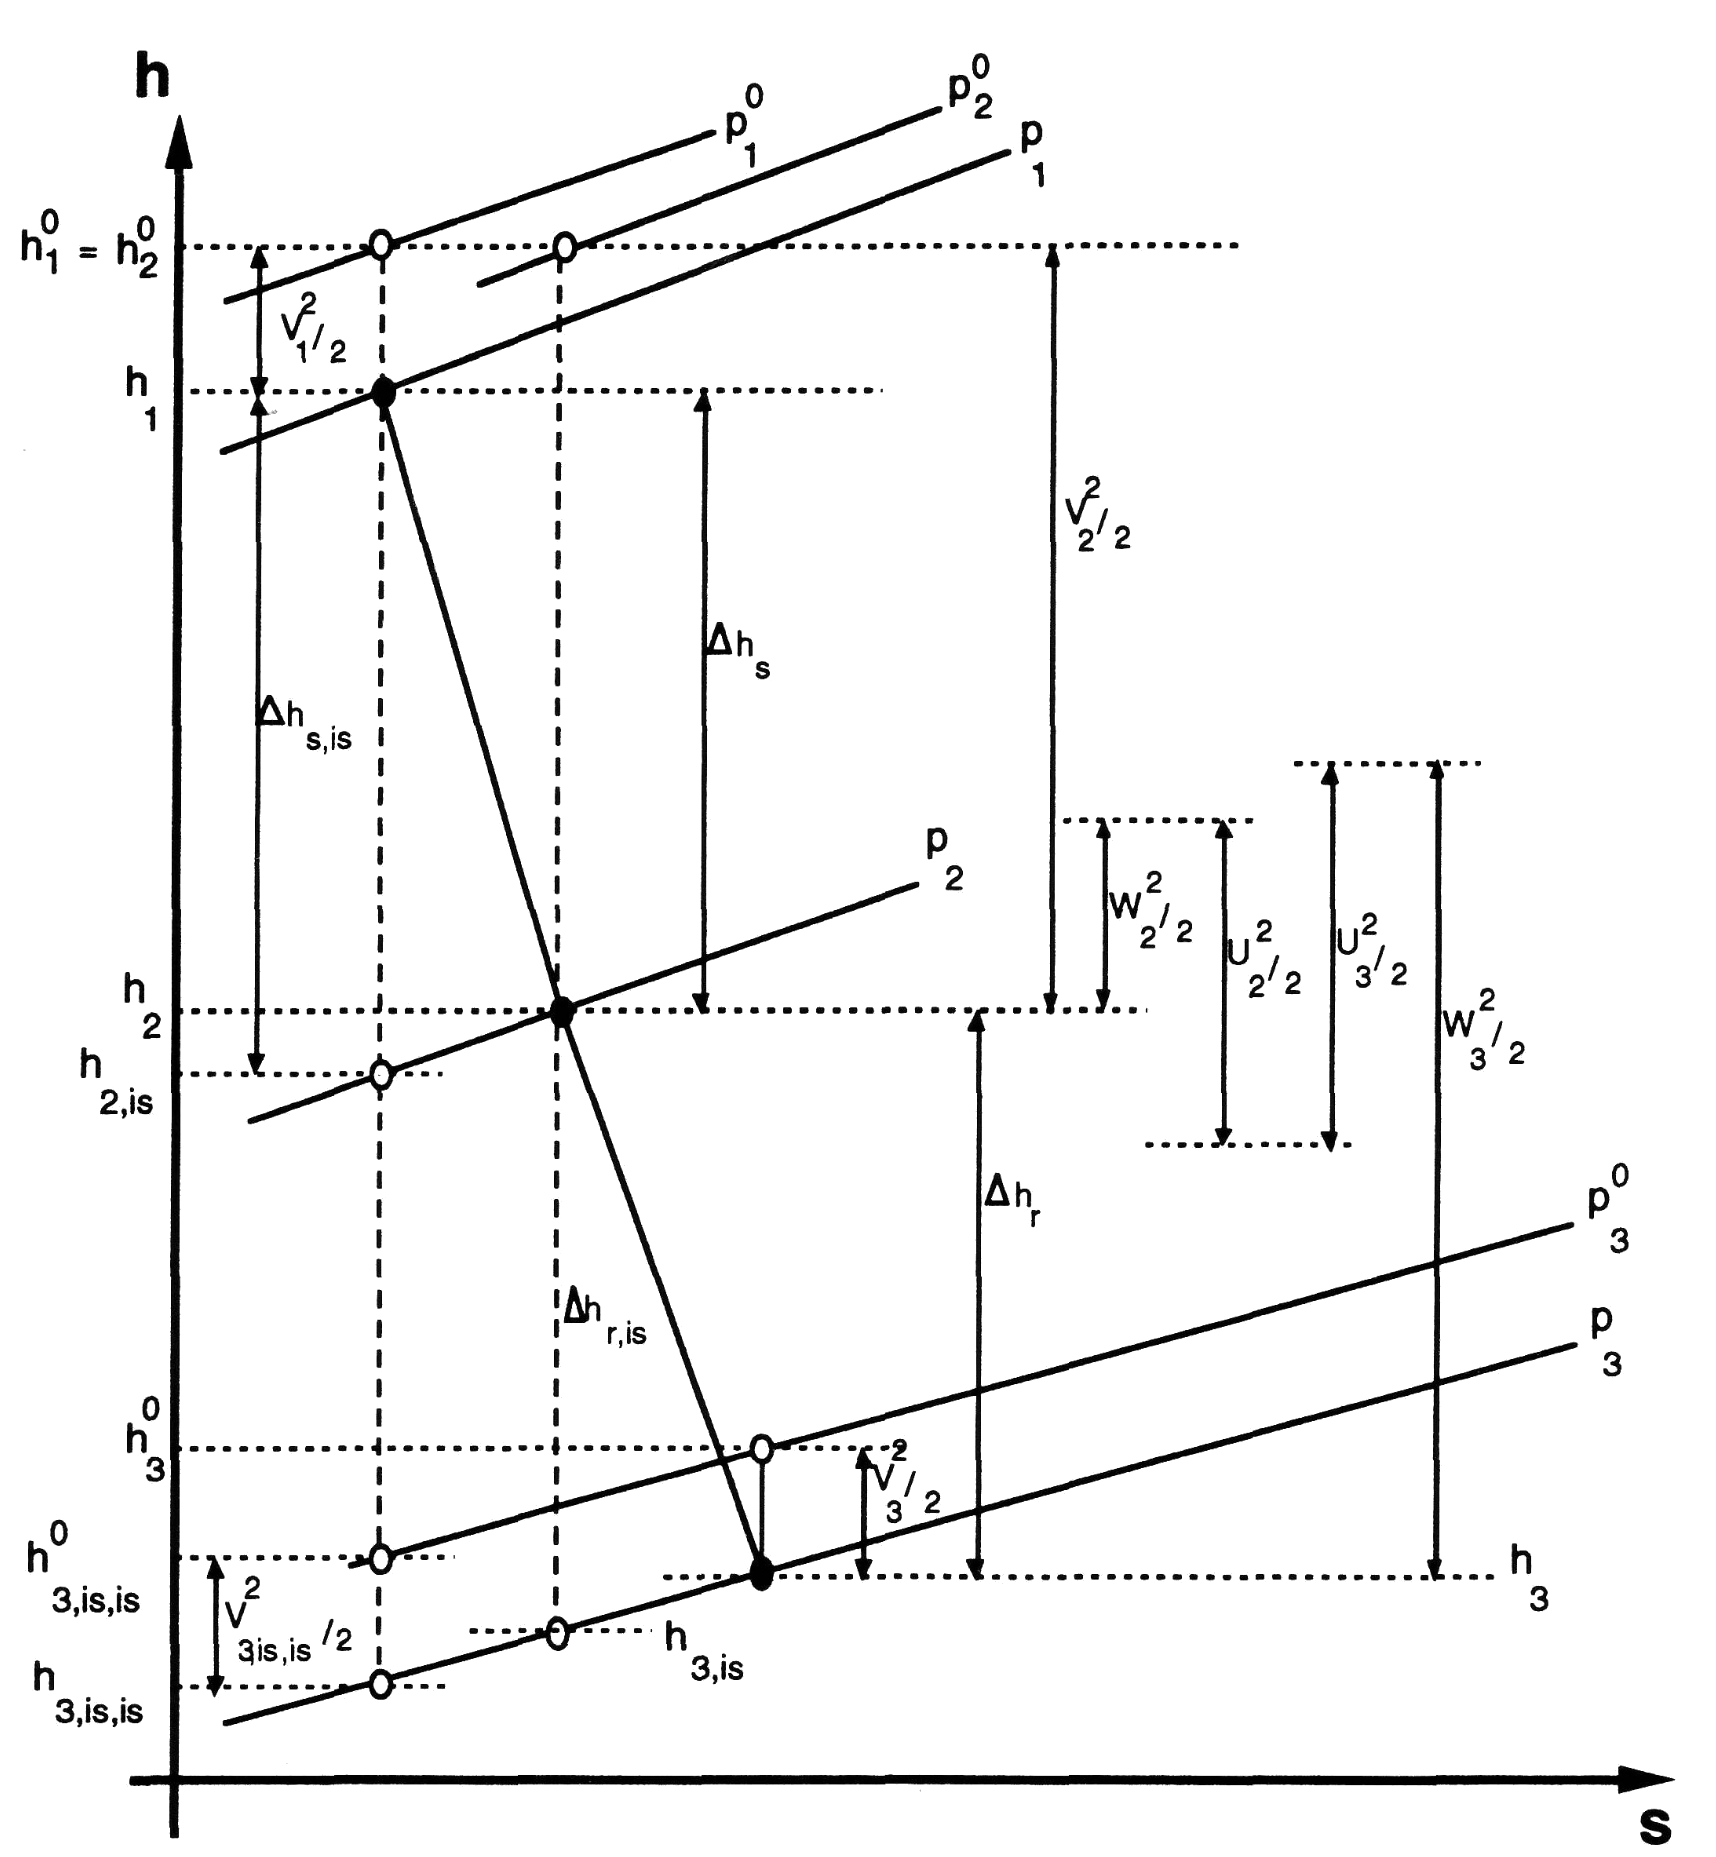
\includegraphics[width=0.5\textwidth]{Turb_mollier.png}
    \caption{Mollier diagram of a turbine stage \cite{Hillewaert2019}.}
    \label{fig:C4_Mollierturb}
\end{figure}

\begin{itemize}
    \setstretch{1}
    \item State \textbf{1}: Starting from the static enthalpy and pressure, the total quantities can be deduced.
    \item State \textbf{2}: The transformation \textbf{1}-\textbf{2} takes place within the stator of the turbine stage. Therefore, the total enthalpy is conserved over the transformation ($h_2^0=h_1^0$).

    Knowing the total enthalpy of the state \textbf{2} allows to compute the static enthalpy and by extension the total rothalpy. Plus, since the flow is accelerated by the stator blades, the static and total pressure falls from state \textbf{1} to state \textbf{2} (\(p_2^{(0)}<p_1^{(0)}\)).
    \item State \textbf{3}: The transformation \textbf{2}-\textbf{3} takes place within the rotor of the turbine stage. Therefore, the total rothalpy is conserved over the transformation (\(i_3^0=i_2^0\)).

    Then, the relation (\ref{eq:C4_i0}) allows retrieving the static enthalpy of state \textbf{3}. As shown on the schematic \ref{fig:C4_turbstage} of the turbine stage, the relative speed of the flow is augmented when going through the rotor passage. This generates a second drop of the static and total enthalpy and pressure (\(p_3^{(0)}<p_2^{(0)}\)).

    However, there exists a special stage for which “the relative velocity of the flow to the blade row” of the rotor\cite{Hillewaert2019} remains unchanged, but the flow is inverted. Neglecting the very small variation of the rotor velocity, the static enthalpy and pressure remains unchanged when passing through the rotor.
\end{itemize}




\subsubsection{Degree of reaction}
\quad\ The last written paragraph mentioned that some turbines are designed to put all the pressure drop over the stator to limit the axial force generated in the rotor.

As a general rule, it is possible to classify the turbomachines by creating two categories based on the degree of reaction \(R\). The degree of reaction is defined as being the ratio between the static enthalpy drop (resp. raise) over the rotor and the static enthalpy drop (resp. raise) over the turbomachine stage.
\begin{equation}
    R = \frac{h_2 - h_3}{h_1 - h_3}\label{eq:C4_R}
\end{equation}
From this definition, the two categories can be defined as follows:

\begin{itemize}
    \setstretch{1}
    \item The impulse or action turbomachines: The degree of reaction \(R\simeq 0\). Thus, since the rotor doesn't see any pressure difference, the axial thrust on the shaft is minimized. 
    \item The reaction turbomachines: The degree of reaction \(R\) is often between 0.5 and 0.7. This means that the pressure drop is distributed between the stator and the rotor.
\end{itemize}

\subsubsection{Performance maps}
\quad\ The turbines can be also be characterized by a performance map determined from experimental results. The map is often composed of two performance plots as shown in the Figure \ref{fig:C4_turbmap}.

\begin{figure}[h]
    \centering
    \includegraphics[width=0.8\textwidth]{Turb_Map.png}
    \caption{Illustration of a turbine performance map \cite{Dixon2013}.}
    \label{fig:C4_turbmap}
\end{figure}

The two plots in the Figure \ref{fig:C4_turbmap} depicts the relations \(\Pi_{tt,t}(\dot{m}_{corr,t},N_{corr,t})\) and \(\eta_t(\Pi_{tt,t},N_{corr,t})\). 

As it can be noticed on the right diagram, all the curves are all stacked on each other when a certain pressure ratio is reached. Compared to the compressor, the choking phenomenon occurs for the same mass flow rate, regardless the rotational speed considered. 

For a turbine, the expansion is mainly performed within its statoric parts. This massive drop of the total pressure comes with a big increase of the kinetic energy of the flow. 

Therefore, it is within this part of the turbine stage that the choking phenomenon will likely occur. Since the stator is not rotating, the maximal mass flow rate is not really impacted by the rotating speed of the rotor. This is the reason why all the iso-rotational speed curves have the same asymptotic value for the mass flow rate.

To summarize what has been seen in this section about turbomachines, the performance map of the compressor and the turbine
have been introduced thanks to the definition of corrected mass flow rate and rotational speed.

Also, the descriptions of the compression and the expansion have been explained using the h-s Mollier diagrams. Those diagrams, along with the schematic of the compressor and turbine stages, allow describing with a decent accuracy the two previously mentioned transformation.

\newpage
\section{Combustion chamber}
%%%%%%%%%%%%%%%%%%%%%%%%%%%%%%%%%%%
%%%%%                         %%%%%
%%%%% <<Combustion chamber>>  %%%%%
%%%%%                         %%%%%
%%%%%%%%%%%%%%%%%%%%%%%%%%%%%%%%%%%
\quad\ The previous section introduced the turbomachines and described those using schematic and h-s diagram. The notion of compressible has been defined, and some important concepts have been emphasized.

In this section, the description of the combustion principle will be considered. Since the study of the fluid mechanic inside the combustion chamber is out of the scope of this work, only combustion equations without dynamic and non-steady effects will be considered.

\subsection{Basis about Chemistry}
\quad\ As it has been mentioned, some combustion reactions will be introduced in this section. Thus, the basic knowledge about chemistry has to be provided.

\subsubsection{Conservation of mass}
During a chemical reaction, the law of conservation of mass (also called the Lavoisier law) has to be satisfied. This implies that the mass of all the reagents combined has to be equal to the mass of the products. An example of chemical reaction is given in (\ref{eq:C4_chem}).

\begin{equation}
    \setstretch{1}
    \underset{\mathrm{16g}}{\ce{1CH4}} \ce{+} \underset{\mathrm{64g}}{\ce{2O2}} \ce{->} \underset{\mathrm{44g}}{\ce{1CO2}} \ce{+} \underset{\mathrm{36g}}{\ce{2H2O}} \ce{+}\text{Heat}\label{eq:C4_chem}
\end{equation}

It will be seen later that this reaction corresponds to the combustion of \textbf{1} mole of methane (\ce{CH4}) using \textbf{2} mole of oxygen (\ce{O2}). The products of the reaction are \textbf{1} mole of \ce{CO2}, \textbf{2} moles of \ce{H2O} and a certain amount of heat transfer to the surroundings. This heat transfer is the desired product of the combustion.

\subsubsection{Conservation of the atomic species}
The second law of conservation states that, during the transformation of the reagent X into the product Y, all the atomic elements from X have to be recovered in Y. For instance, for the equation (\ref{eq:C4_chem}), there is one mole of carbon (\ce{C}) in the reagents. Thus, one mole of \ce{C} has to be present in the products of the reaction.
\newpage
\subsubsection{Proust's law}
The third law to be considered is the Proust law which states that for each chemical reactions, ''the ratio between the mass of each reagent is a constant''. Considering the above example (\ref{eq:C4_chem}), the ratio between the mass of \ce{O2} and \ce{CH4} consumed is given in the equality (\ref{eq:C4_O2CH4mass})

\begin{equation}
    \setstretch{1}
    \frac{\text{mass of \ce{O2} consumed}}{\text{mass of \ce{CH4} consumed}} = 4 \label{eq:C4_O2CH4mass}
\end{equation}

Let's remark that the law is also valid considering the consumed quantities in mole. In molar quantities, the relation (\ref{eq:C4_O2CH4mass}) becomes (\ref{eq:C4_molratio}).

\begin{equation}
    \setstretch{1}
    \frac{\text{mole of \ce{O2} consumed}}{\text{mole of \ce{CH4} consumed}} = 2  \label{eq:C4_molratio}
\end{equation}

This ratio depends on the type of fuel used. For instance, if the fuel were propane (\ce{C4H8}), the ratio would be equal to 5.

\subsection{Combustion equation}
\quad\ The equation \ref{eq:C4_chem} was illustrating the combustion of the methane \ce{CH4}. The reaction, as written there, supposed that amount of oxygen provided for the reaction is just enough to consume all the methane injected.

This situation, which is the reference, is characterized by an air factor \(\lambda = 1\) (or an excess of air \(e=\lambda-1=0\)). It is said that such combustion is at the stoichiometry.

\subsubsection{Air factor}
The air factor is then defined as being the ratio between

\begin{equation}
    \setstretch{1}
    \lambda = \frac{\varkappa}{\varkappa_{\left.\right|stoichiometry}} \label{eq:C4_lbd}
\end{equation}
Where $\varkappa \doteq \frac{\text{mole of \ce{O2} consumed}}{\text{mole of fuel consumed}}$
Let's note that every other combustive can replaced the oxygen in the relation. However, \ce{O2} is the most common one. Thus, the following development will not consider this possibility.
For the following, the notation \(w_{\ce{\text{<molecules>}}}\) will be used in replacement for ''mole of <molecules> consumed''.

\begin{equation}
    \setstretch{1}
    \lambda = \frac{w_{\ce{O2}}}{2\cdot w_{\ce{CH4}}}\label{eq:C4_lbdCH4}
\end{equation}

For the case of the \ce{CH4} being the fuel, it has been shown in the previous section that the value of the denominator of relation (\ref{eq:C4_lbd}) is equal to 2. Therefore, for this particular combustion, the relation (\ref{eq:C4_lbdCH4}) defines the air factor.



\subsubsection{Generalized combustion equation}
\quad\ As explained, the chemical reaction (\ref{eq:C4_chem}) represents the ideal case with an air factor of 1. Also, it is considered that the combustive is pure \ce{O2}. In reality, the used reagent for the combustion is ambient air which is composed of 21\% of \ce{O2} and 79\% of \ce{N2} (nitrogen).

Thus, the generalized combustion equation (for the \ce{CH4}) is defined as in the reaction (\ref{eq:C4_chemgeng0}).

\begin{equation}
    \setstretch{1}
    \ce{CH4 +}2\lambda \left(\ce{O2}+\frac{79}{21}\ce{N2}\right) \ce{-> CO2 + 2(\lambda-1)O2 + 2H2O + 2\lambda\frac{79}{21}N2 + \text{Heat}}\label{eq:C4_chemgeng0}
\end{equation}

This equation, while being correct for any values of \(\lambda\) greater or equal than 1, has to be modified to take into account the event for which the excess of air \(e\) is lower than zero (with \(e=\lambda -1\)). For such values, the combustion equation then becomes as stated in (\ref{eq:C4_chemgeng1}).

\begin{equation}
    \setstretch{1}
    \ce{CH4 +}2\lambda \left(\ce{O2}+\frac{79}{21}\ce{N2}\right) \ce{-> aCO2 + bCO + 2H2O + 2\lambda\frac{79}{21}N2 + \text{Heat}}\label{eq:C4_chemgeng1}
\end{equation}

where coefficients ''a'' and ''b'' satisfies the system (\ref{eq:C4_sysab})

\begin{equation}
    \setstretch{1}
    \begin{cases}
        \text{a} + \text{b} = 1 \\
        2\text{a} + \text{b} = 4\lambda - 2
    \end{cases}\label{eq:C4_sysab}
\end{equation}

Where both equations have been obtained based on the conservation of the atomic species. It can be calculated that there exists a lower bound for the air factor below which the combustion will be impossible. The condition is that the coefficient ''a'' cannot be smaller than zero. For this case, the minimal air factor \(\lambda_{min} =-\frac{3}{4}\).

To provide some definitions, the mixture \ce{O2}-fuel is said poor when \(\lambda>1\), rich when \(\lambda<1\) and at the stoichiometry for an air factor \(\lambda=1\). Typically, for a gas turbine the mixture is very poor with a $\lambda$ often greater than 4-5.

\subsection{Fuel characteristic}
\quad\ From now, the amount of heat provided during the combustion has not been quantified. This quantification is really important because this amount of heat is linked to quality and the nature of the fuel.

\subsubsection{Heating calorific value}
\quad\ First, let's define the heating calorific value \(HCV\) of a fuel (J/kg). By definition, it is ''the amount of thermal energy released during the total combustion of one physical unit of fuel” \cite{Leonard2018}.

\begin{equation}
    \setstretch{1}
    HCV = -\Delta H^o_{combustion} \label{eq:C4_HCV1}
\end{equation}

With \(-\Delta H^o_{combustion}\) being the heat released during the reaction.

The \(HCV\) is determined at a given reference temperature \(T_0\). Considering this reference temperature, the \(HCV\) can be evaluated by computing the enthalpy difference between the reagents and the products.

\begin{equation}
    \setstretch{1}
    HCV = h_{reagent\left.\right|T=T_0} - h_{product\left.\right|T=T_0}\label{eq:C4_HCV2}
\end{equation}

Distinction between the lower and higher heating calorific value (respectively $HCV_l$ and $HCV_h$) have to be made. Basically, when considering the combustion of a given fuel, the amount of energy released corresponds to the lower heating calorific value if the water remains gaseous within the exhaust gas. 

However, when the water contained in the exhaust gas have been condensed into liquid water, the energy released from the phenomenon is added to the lower HCV. For this case, the higher heating calorific value is then used instead of the lower one.  

The \(HCV\) value depends on the type of fuel that is used. For example, the lower heating calorific value of the \ce{CH4} is around 50 MJ/kg.

\subsubsection{Adiabatic flame temperature}
\quad\ The second notion that can be defined is the adiabatic flame temperature \(T_f\). If the combustion chamber is supposed to be adiabatic (no heat transfer to the outside), the heat generated will be fully retained within the exhaust gas of the combustor. Thus, the temperature reached by the gas is considered to maximal and is called the adiabatic flame temperature.

The evaluation of the temperature \(T_f\) is quite similar to the one of the \(HCV\). Here, starting from the reference temperature, the temperature \(T_f\) is calculated such that the enthalpy of the products is equal to the enthalpy of the reagents.

\begin{equation}
    \setstretch{1}
    \left.h_{reagent}\right|_{T=T_0} = \left.h_{product}\right|_{T=T_f}\label{eq:C4_T_f}
\end{equation}

\subsubsection{Combustion efficiency}
\quad\ The combustion efficiency is defined as being the ratio between the heat injected into the combustion chamber the heat that can be \textit{used} for the combustion. This is expressed in the relation (\ref{eq:C4_etaCC}).

\begin{equation}
    \setstretch{1}
    \eta_{cc} = \frac{\dot{Q}}{\dot{m}_{Fuel}\cdot HCV_{Fuel}}\label{eq:C4_etaCC}
\end{equation}
\subsection{Fumes composition}
\quad\ Previously has been presented in the equations (\ref{eq:C4_chemgeng0}) and (\ref{eq:C4_chemgeng1}) the generalized chemical reaction for the combustion of the methane.
In a more general case, if the fuel is essentially composed of carbon \ce{C}, hydrogen \ce{H}, oxygen \ce{O} and nitrogen \ce{N}, the reactions (\ref{eq:C4_chemgeng0}) and (\ref{eq:C4_chemgeng1}) can be reformulated taking into account a general composition for the fuel.

\begin{subequations}
    \setstretch{1}
 \begin{align}
     \ce{C_{\text{m}}H_{\text{n}}O_{\text{x}}N_{\text{y}} +}\kappa\lambda \left(\ce{O2}+\frac{79}{21}\ce{N2}\right) &\ce{-> mCO2 +} \kappa(\lambda-1)\ce{O2 + \frac{n}{2}H2O +} (\kappa\lambda\frac{79}{21} + \frac{\text{y}}{2})\ce{N2}\\
     \text{ for \(\lambda\geq 1\)}\nonumber\\
     \ce{C_{\text{m}}H_{\text{n}}O_{\text{x}}N_{\text{y}} +}\kappa\lambda \left(\ce{O2}+\frac{79}{21}\ce{N2}\right) &\ce{-> aCO2 + bCO + \frac{n}{2}H2O} + (\kappa\lambda\frac{79}{21} + \frac{\text{y}}{2})\ce{N2}\\
     \text{ for \(\lambda< 1\)}\nonumber
 \end{align}
        \label{eq:C4_chemgeng01}
\end{subequations}

where coefficients ''a'' and ''b'' satisfies the system (\ref{eq:C4_sysab2})

\begin{equation}
    \setstretch{1}
    \begin{cases}
        \text{a} + \text{b} = \text{m} \\
        2\text{a} + \text{b} = 2\kappa\lambda + \frac{\text{x}}{2} - \frac{\text{n}}{2}
    \end{cases}\label{eq:C4_sysab2}
\end{equation}

With the factor \(\kappa = (\text{m}+\frac{\text{n}}{4}-\frac{\text{x}}{2})\). The coefficients ''m'' and ''n'' correspond to the number of moles of atoms of carbon and hydrogen within one mole of fuel.

From theses equations, it is possible to obtain the molar fraction \(x_i\) of each fume components. By definition, the molar fraction of the component \(i\) is the ratio between the number of moles \(n_i\) of the component \(i\) and the total number of moles \(n_{tot}\), all species taken together.

\begin{equation*}
    \setstretch{1}
    x_i = \frac{n_i}{n_{tot}}
\end{equation*}

From the molar fraction, the mass fraction can be obtained using the formula (\ref{eq:C4_x2y})

\begin{equation}
    \setstretch{1}
    y_i = x_i\frac{MM_{tot}}{MM_i} \label{eq:C4_x2y}
\end{equation}

Where \(MM_i\) is the molar mass (in g/mol) of the component \(i\) and \(MM_{tot}\) is the total molar mass of the fumes. The total molar mass of the fumes is obtained as stated in the relation (\ref{eq:C4_MMtot}).

\begin{equation}
    \setstretch{1}
    MM_{tot} = \sum_i x_i\cdot MM_i \label{eq:C4_MMtot}
\end{equation}

This method will be called the ''weight factor'' method.

\section{Heat-exchangers}
%%%%%%%%%%%%%%%%%%%%%%%%%%%%%%%%%%%
%%%%%                         %%%%%
%%%%%   <<Heat-exchanger>>    %%%%%
%%%%%                         %%%%%
%%%%%%%%%%%%%%%%%%%%%%%%%%%%%%%%%%%
\quad\ The last important component that has to be defined and characterized is the heat exchanger (HX). As the name says, the purpose of this element is to transfer the heat from a \textbf{hot} fluid to a \textbf{cold} fluid. The heat-exchangers can be classified into several categories\cite{Ngendakumana2018}.

\begin{itemize}
    \setstretch{1}
    \item The recuperators: their purpose is to recover the heat from a hot fluid to heat up a cold fluid for direct usage. For instance, the exhaust gas from a boiler will go through a recuperator to exchange its energy with water. For this application and for many others, the two streams within the HX are separated by physical walls.

    Alternatively, the heat exchange can be performed by direct contact between the two fluids. In this case, nothing prevents the hot flow from mixing with the cold flow (and vice versa).
    \item The regenerators: considering a cycle , the purpose of the regenerators is to use a hot flow from the cycle to heat up a cold flow from the same cycle.
\end{itemize}

By definition, the hot stream is the one that \textbf{provides} the heat, and the cold stream is the one \textbf{receiving} the heat.

In the Figure \ref{fig:C4_HX} are depicted some illustrations of heat exchanger owning at different families.
\begin{figure}[h]
    \centering
    \subfloat[HX with fined plates\cite{Ngendakumana2018}.\label{fig:C4_HX_fin_plate}]
    {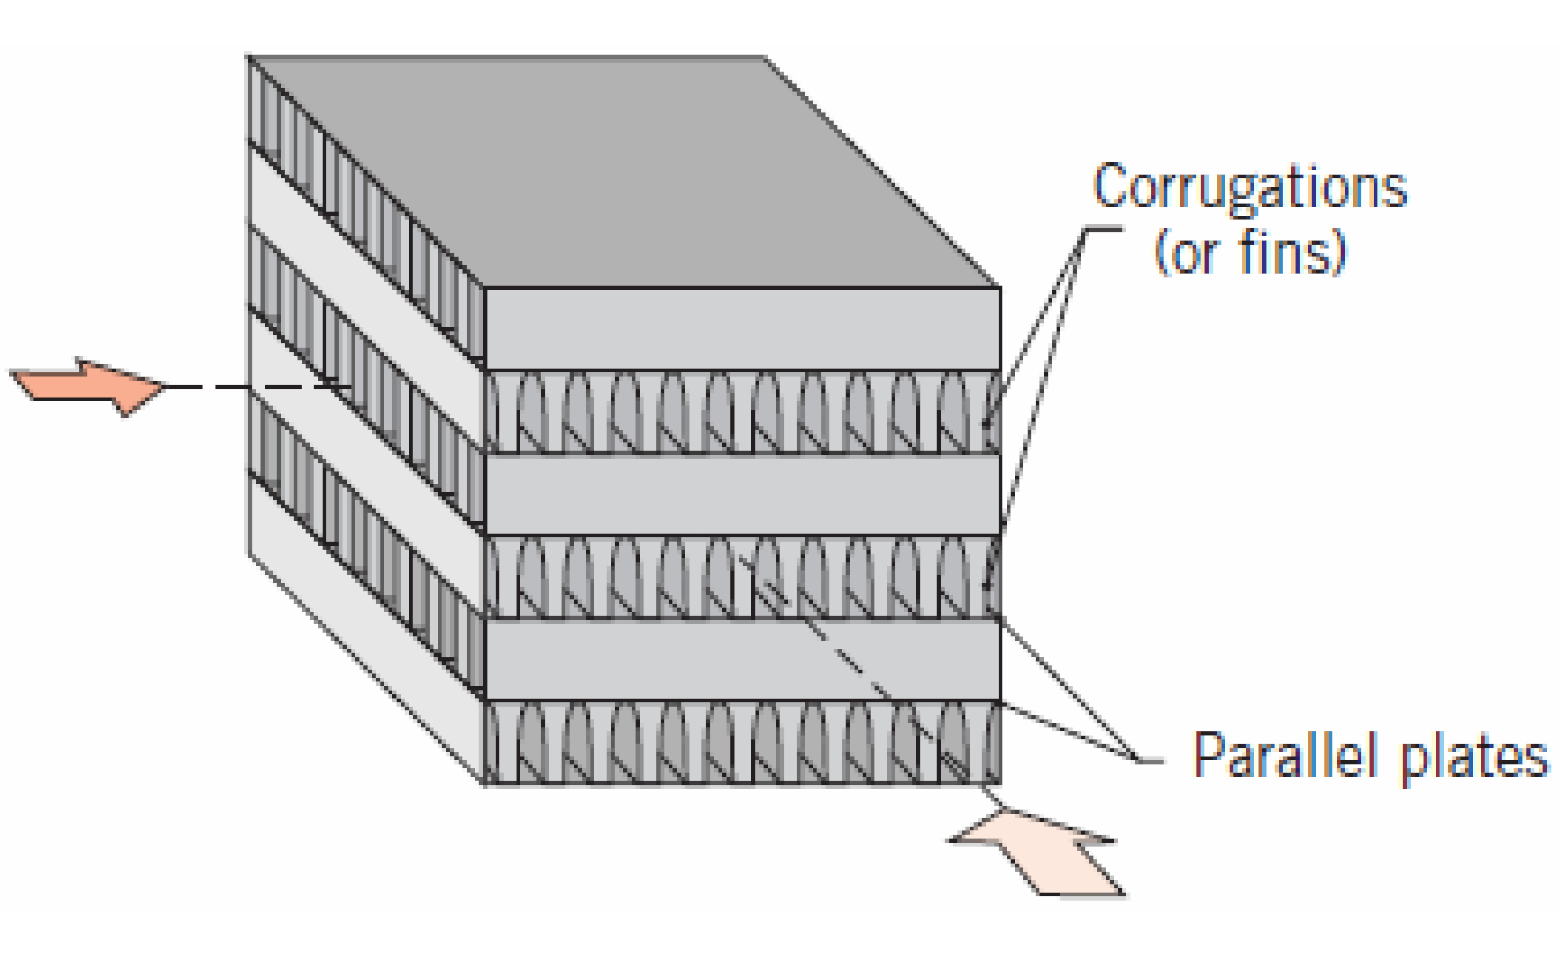
\includegraphics[width=0.4\textwidth]{HX_fin_plate}}\hfill
    \subfloat[HX with fined tubes \cite{Ngendakumana2018}.\label{fig:C4_HX_fin_tube}]
    {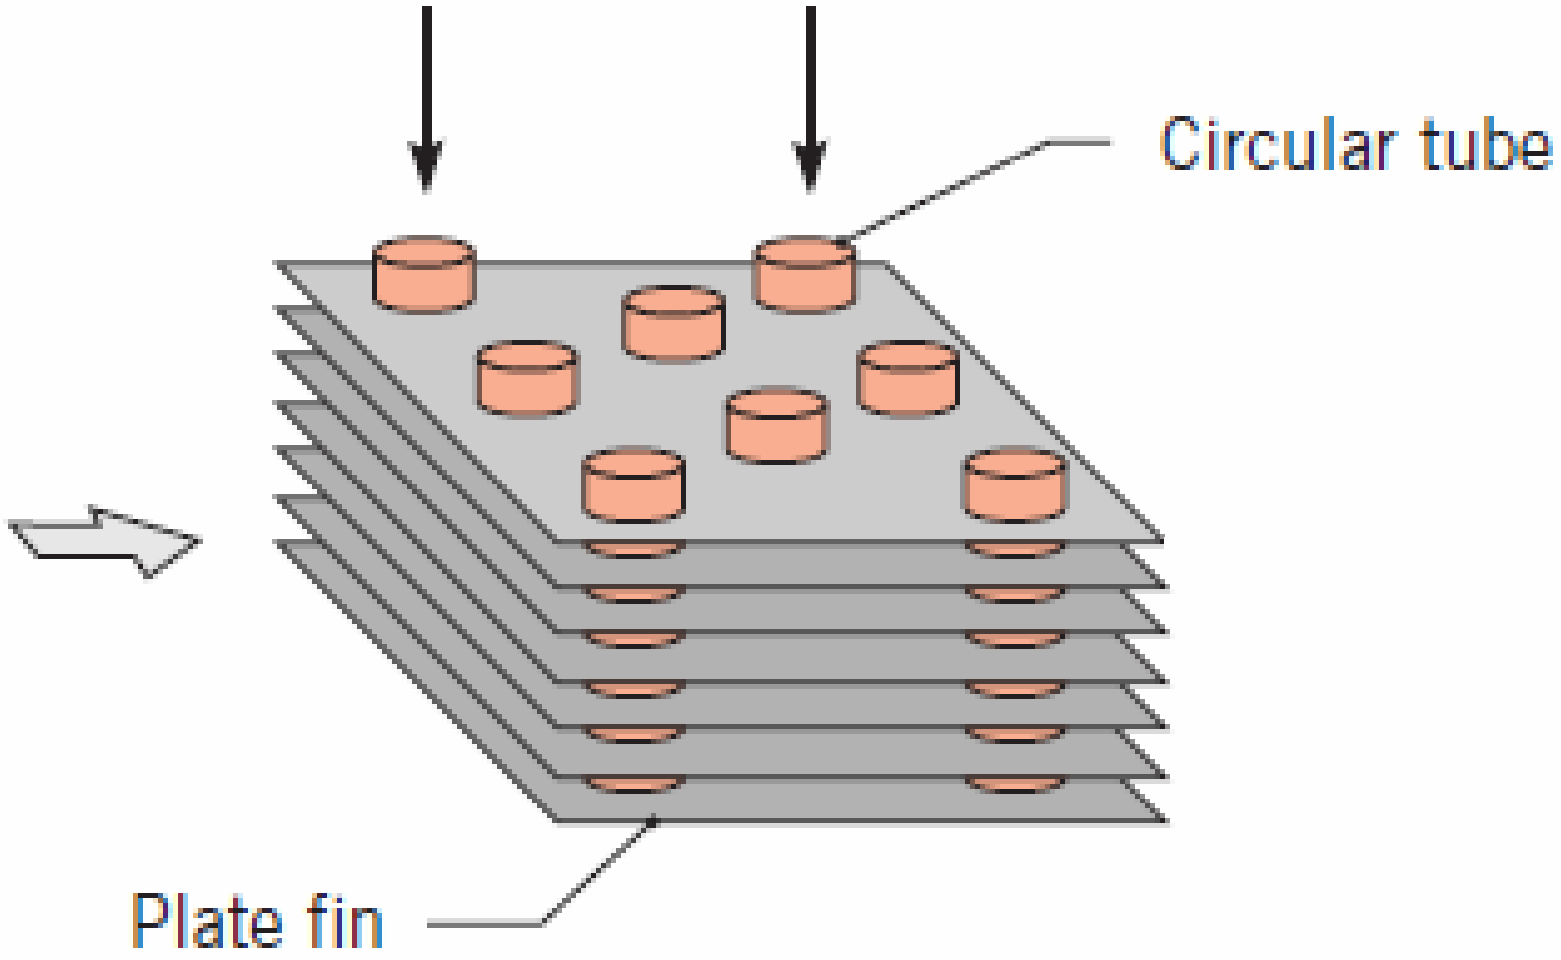
\includegraphics[width=0.4\textwidth]{HX_fin_tube}}\hfill
    \subfloat[Plate heat exchangers\cite{Ngendakumana2018}.\label{fig:C4_PHE}]
    {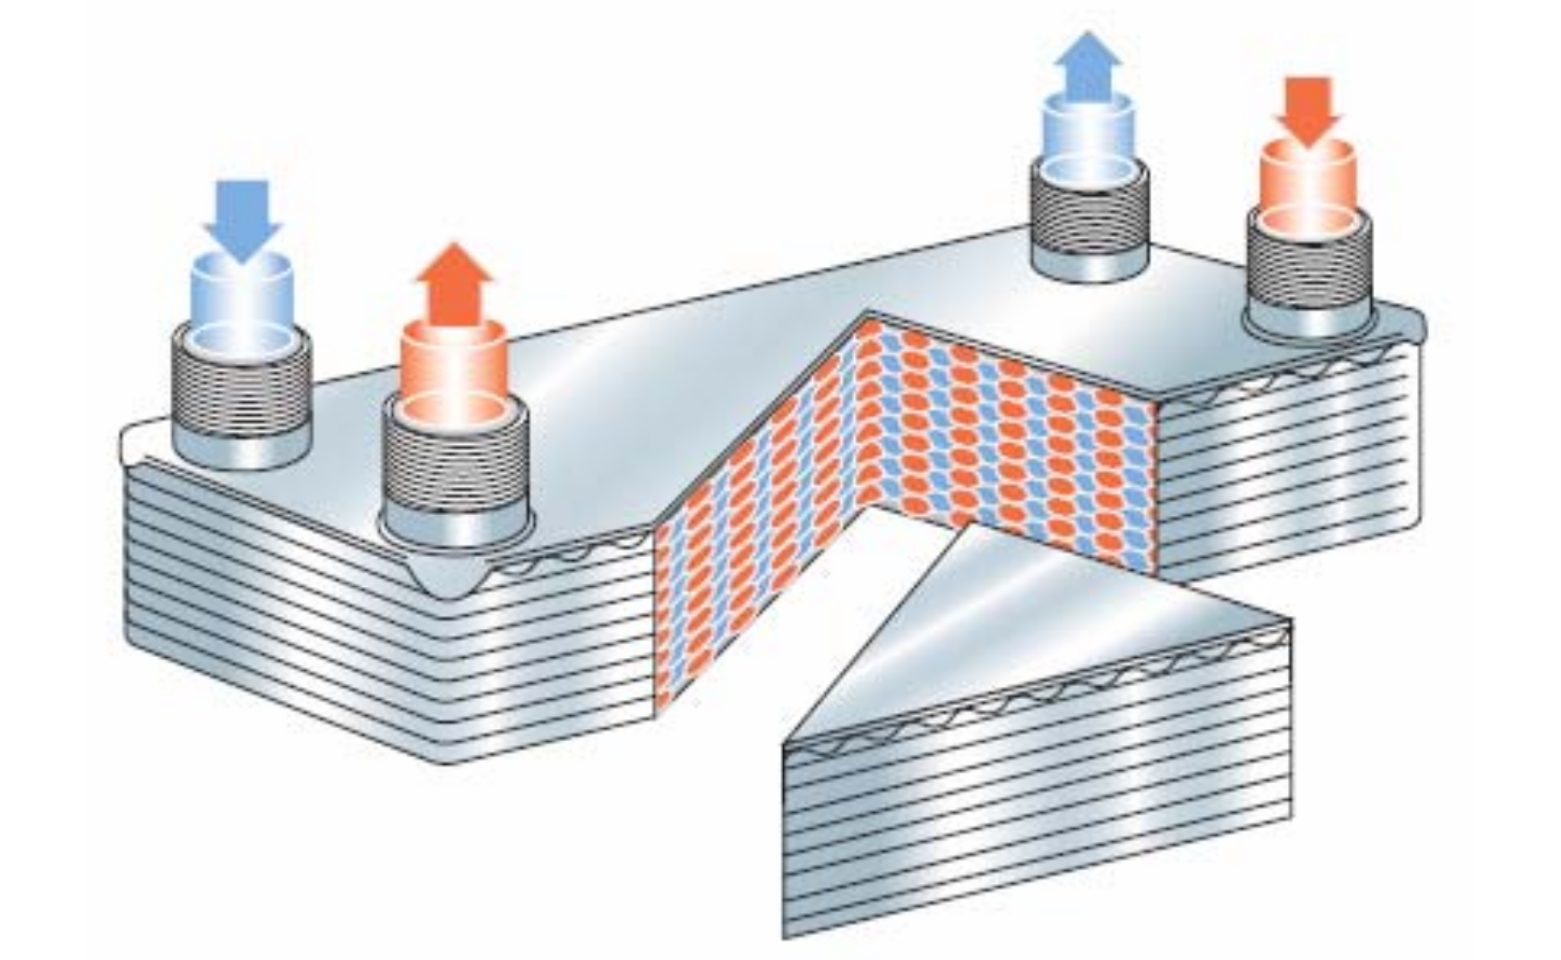
\includegraphics[width=0.4\textwidth]{HX_brased_plate}}
    \caption{HX illustrations.} \label{fig:C4_HX}
\end{figure}

The selected family will highly depends on the type of application that is targeted. Plate heat exchangers are one of the most compact types of heat exchangers. This compactness is highly appreciated for any system where the foot print and volume have to be as minimal as possible. However, this is at the cost of more complicated maintenance due to the brazing of the plates.

This section will not cover the specificity of these different families. Instead, the main notions which are necessary to characterize the heat transfer between two fluids will be given.

\subsection{Stream configurations}
\quad\ There isn't a unique configuration regarding about the interaction between the hot and cold streams. Indeed, here are the main categories based on flow configurations.

\begin{itemize}
    \setstretch{1}
    \item Parallel flow HX: The two streams go through the heat exchanger in the same direction (Figure \ref{fig:C4_para_flow}).

    \item Counter flow HX: The two streams go through the heat exchanger in the opposite direction. This configuration is more frequent than the parallel flow HX due to higher efficiency. However, sometimes the network of piping doesn't permit installing such configuration (Figure \ref{fig:C4_counter_flow}).

    \item Cross flow HX, both fluids unmixed: The flow in the tube does not see the property of cross flow varying along with the distance traveled. Both flows are unmixed (Figure \ref{fig:C4_cross_flow_unmixed}).
  
    \item Cross flow HX, one fluid mixed: The flow in the tube does not see the property of cross flow varying along with the distance traveled. The cross flow does not travel inside isolated channels (Figure \ref{fig:C4_cross_flow_1mixed}).
\end{itemize}
\begin{figure}[h]
    \centering
    \begin{subfigure}[b]{0.4\textwidth}
        \centering
        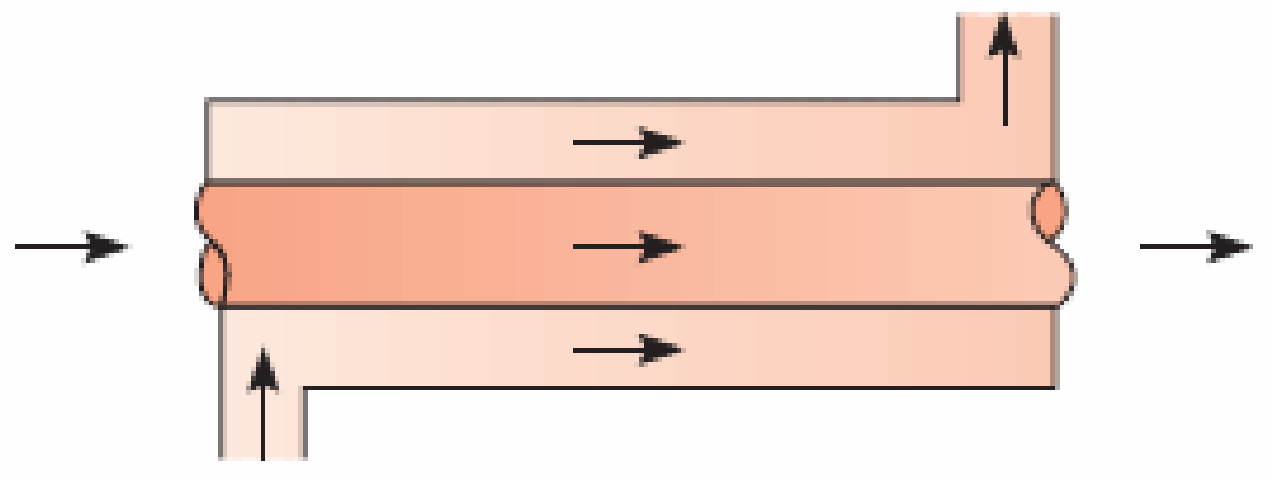
\includegraphics[width=\textwidth]{parallele_flow}
        \caption{Parallel flow heat exchanger \cite{Ngendakumana2018}.}
        \label{fig:C4_para_flow}
    \end{subfigure}
    \begin{subfigure}[b]{0.4\textwidth}
        \centering
        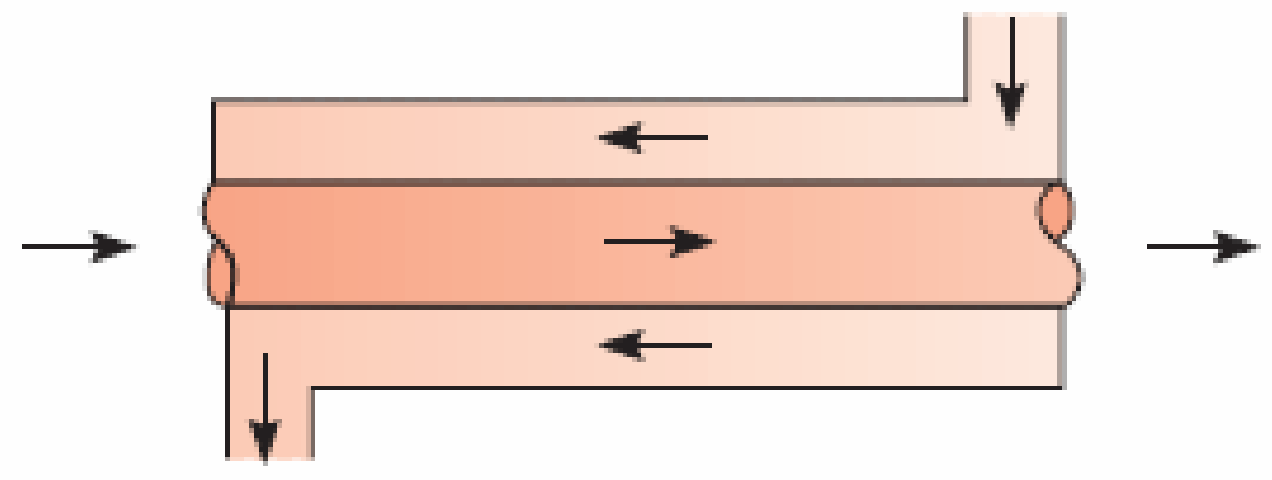
\includegraphics[width=\textwidth]{opposite_flow}
        \caption{Counter flow heat exchanger \cite{Ngendakumana2018}.}
        \label{fig:C4_counter_flow}
    \end{subfigure}
    \begin{subfigure}[b]{0.4\textwidth}
        \centering
        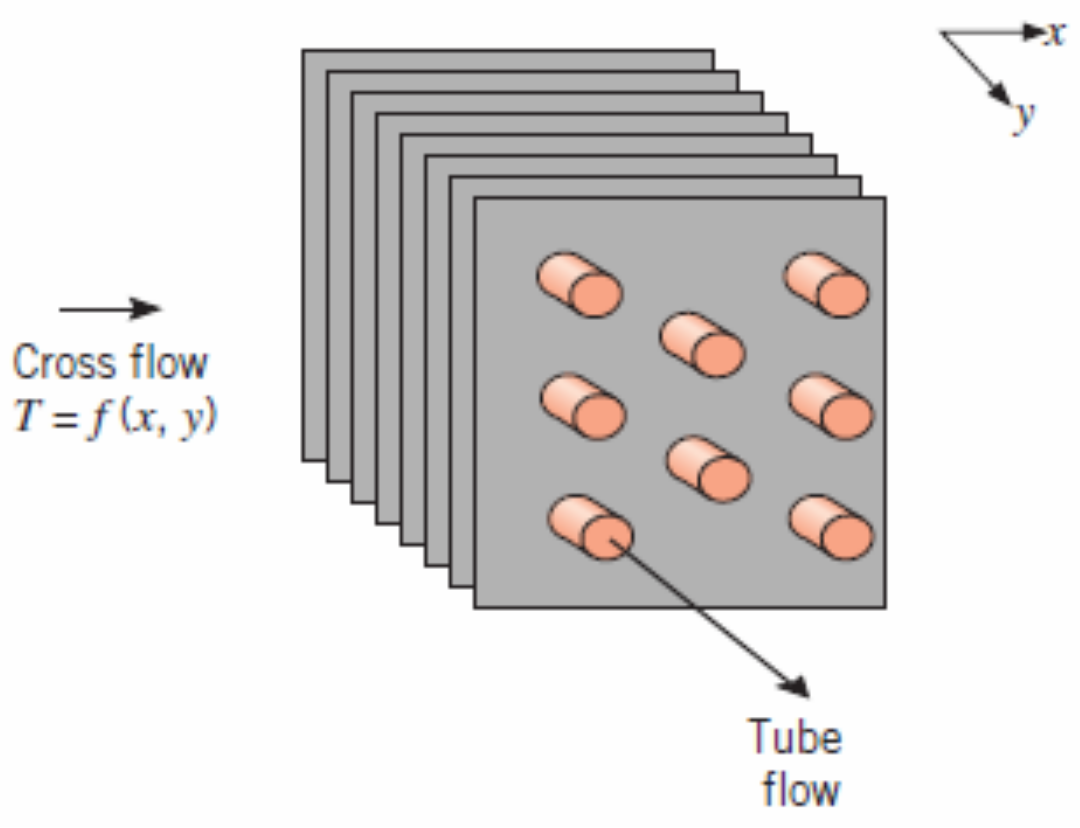
\includegraphics[width=\textwidth]{crossed_flow_non_mixed}
        \caption{Cross flow heat exchanger, both fluids unmixed \cite{Ngendakumana2018}.}
        \label{fig:C4_cross_flow_unmixed}
    \end{subfigure}
    \begin{subfigure}[b]{0.4\textwidth}
        \centering
        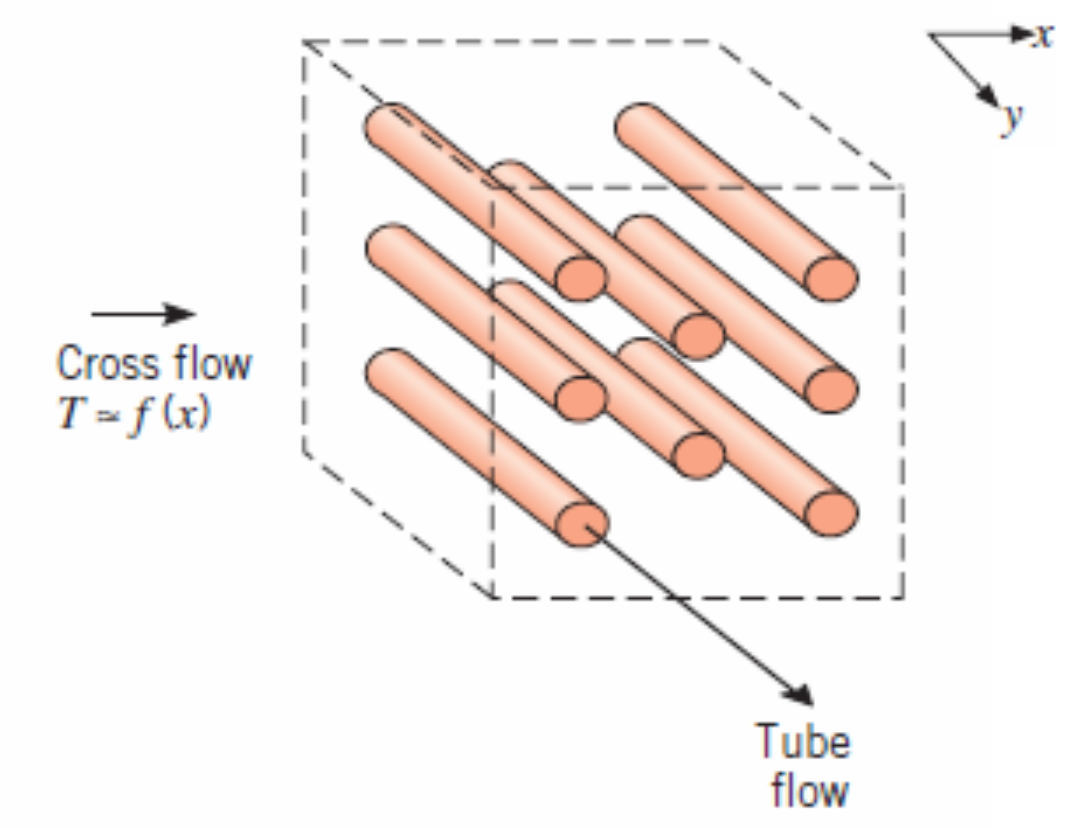
\includegraphics[width=\textwidth]{crossed_flow_one_mixed}
        \caption{Cross flow heat exchanger, one fluid mixed \cite{Ngendakumana2018}.}
        \label{fig:C4_cross_flow_1mixed}
    \end{subfigure}
    \caption{Configuration Heat-exchangers.} \label{fig:C4_config}
\end{figure}
Considering the parallel and counter flow heat exchanger, two temperature differences can be defined based on the temperature profiles (Figure \ref{fig:C4_Tprof}) of both fluids inside the heat exchanger.

\begin{figure}[h]
    \centering
    \begin{subfigure}[b]{0.45\textwidth}
        \centering
        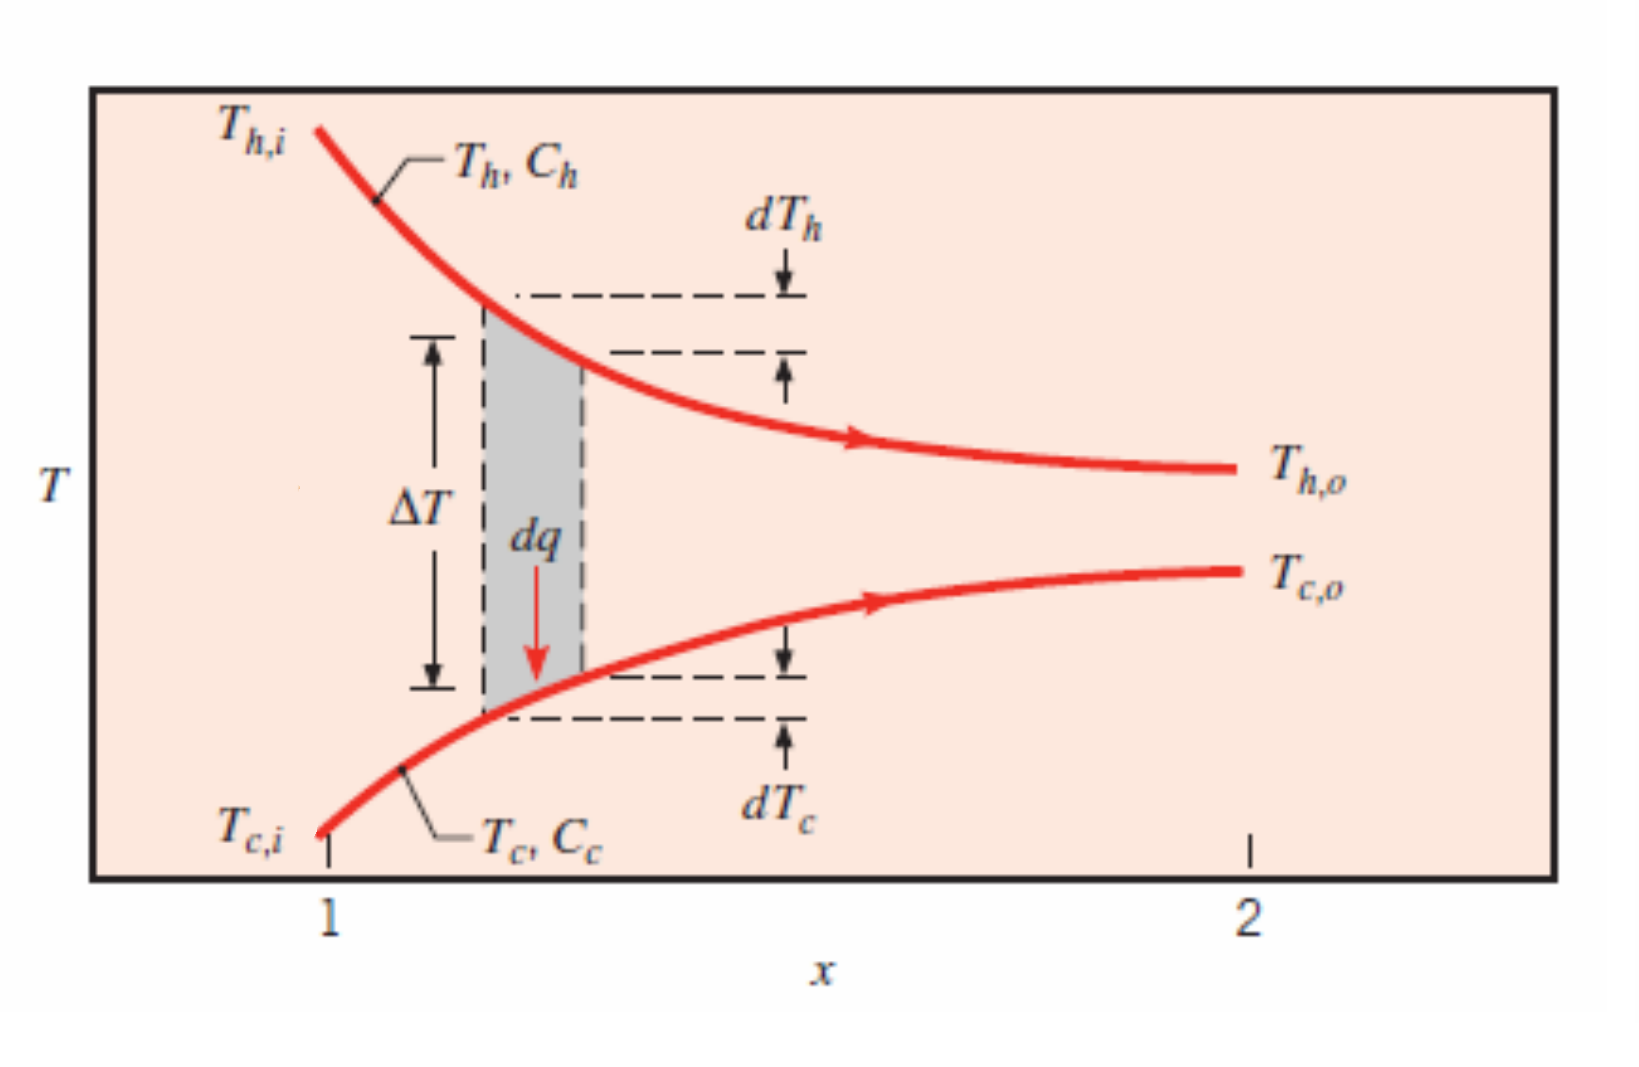
\includegraphics[width=\textwidth]{parallele_flow_T}
        \caption{Temperature profile for parallel flow HX \cite{Ngendakumana2018}.}
        \label{fig:C4_HX_par_flow_T}
    \end{subfigure}
    \begin{subfigure}[b]{0.45\textwidth}
        \centering
        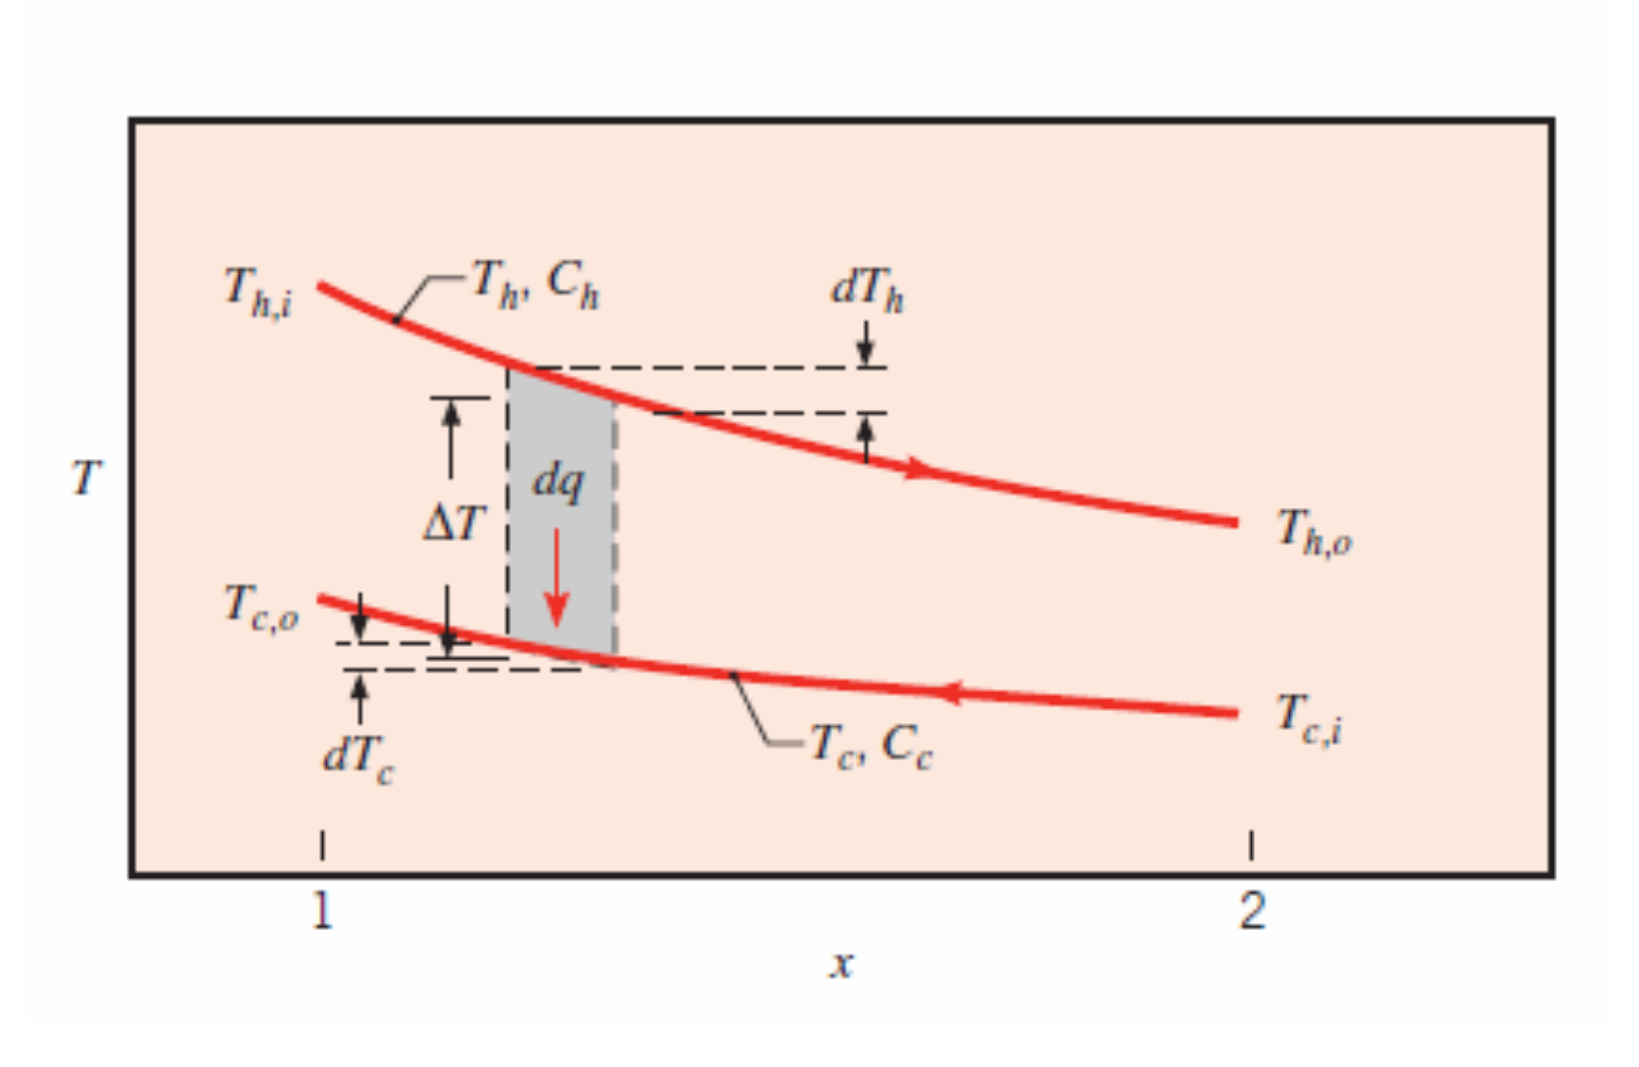
\includegraphics[width=\textwidth]{opposite_flow_T}
        \caption{Temperature profile for counter flow HX \cite{Ngendakumana2018}.}
        \label{fig:C4_HX_opo_flow_T}
    \end{subfigure}
    \caption{Temperature profiles for different stream configurations.}
    \label{fig:C4_Tprof}
\end{figure}

The subscripts $h$ and $c$ indicate which flow is considered (respectively the hot and the cold flow). The subscripts $i$ and $o$ refer to the inlet and the outlet of the heat exchanger.

The first temperature difference \(\Delta T_0\) is defined as being the largest temperature difference between the two flows, regardless of the position inside the HX. Thus, depending on the flow configuration, the \(\Delta T_0\) is given by (\ref{eq:C4_DT0}).

\begin{equation}
    \setstretch{1}
    \Delta T_0 =
    \begin{cases}
        T_{h,i} - T_{c,i} \text{ For the parallel flow} \\
        T_{h,i} - T_{c,o} \text{ For the counter flow}  \\
    \end{cases}\label{eq:C4_DT0}
\end{equation}

The second temperature difference \(\Delta T_L\) corresponds to the smallest temperature difference between the two flows. Similarly to \(\Delta T_0\), \(\Delta T_L\) is defined by the relation (\ref{eq:C4_DTL}).

\begin{equation}
    \setstretch{1}
    \Delta T_L =
    \begin{cases}
        T_{h,o} - T_{c,o} \text{ For the parallel flow} \\
        T_{h,o} - T_{c,i} \text{ For the counter flow}  \\
    \end{cases}\label{eq:C4_DTL}
\end{equation}

\subsection{Heat transfer within a heat exchanger}
\quad\ The heat transfer rate of a heat exchanger is directly dependent on the nature of the fluids and the heat exchanger itself. Let's consider the following relation (\ref{eq:C4_Qdot1})
\begin{equation}
    \dot{Q} = \frac{\Delta T_{LM}}{\mathrm{R}}= \mathrm{A}\cdot \mathrm{U}\cdot \Delta T_{LM}\label{eq:C4_Qdot1}
\end{equation}
Where \(\mathrm{A}\) is the global heat transfer area of the HX, and \(\mathrm{R}\) and \(\mathrm{U}\) are the global thermal resistance and heat transfer coefficient respectively. The difference of temperature \(\Delta T_{LM}\) is called the logarithmic mean temperature difference. Its definition is (\ref{eq:C4_lmtd}).


\begin{equation}
    \setstretch{1}
    \Delta T_{LM} = \frac{\Delta T_0-\Delta T_L}{ln\left(\frac{\Delta T_0}{\Delta T_L}\right)}\label{eq:C4_lmtd}
\end{equation}
With \(ln\) being the neperian logarithm.
\subsubsection{Transfer coefficient}
\quad\ The general definition of the product \(\mathrm{A}\cdot \mathrm{U}\) is written in the equation (\ref{eq:C4_AU}).
 
\begin{equation}
    \setstretch{1}
    \frac{1}{\mathrm{A}\cdot \mathrm{U}}  = \frac{1}{\eta_{0,C}\cdot h_{conv,C} \cdot A_C} + \frac{F_C}{\eta_{0,C}\cdot A_C} + R_w + \frac{F_H}{\eta_{0,H}\cdot A_H} + \frac{1}{\eta_{0,H}\cdot h_{conv,H} \cdot A_H}\label{eq:C4_AU}
\end{equation}
Where \(h_{conv}\) is the convective heat transfer coefficient (W/m$^2\cdot$K) of the fluid, \(F\) is a degradation factor due to the clogging, \(\eta_0\) is the global efficiency of the surface and \(R_w\) is the wall resistance.

Making the assumption that all the ducts considered in this work are smooth and the flows are turbulent, the convective heat transfer coefficient \(h_{conv}\) is obtained using the formula (\ref{eq:C4_h}).
\begin{equation}
    h_{conv} = Nu \cdot \frac{\lambda_c}{D_t} = 0.023\cdot Re^{0.8}\cdot Pr^{1/3}\frac{\lambda_C}{D_t}\label{eq:C4_h}
\end{equation}
Where \(Nu\), \(Re\) and \(Pr\) are respectively the Nusselt, Reynolds and Prandtl number. \(\lambda_c\) is the thermal conductivity (W/m$\cdot$K) of the fluid and \(D_t\) is the diameter of the duct\cite{Ngendakumana2018}.

By definition, the Reynolds and Prandtl numbers are defined as follows
\begin{align}
    Re & = \frac{\rho\cdot v\cdot D_h}{\mu}\label{eq:C4_Re} \\
    Pr & = \frac{\mu\cdot c_p}{\lambda_c}\label{eq:C4_Pr}
\end{align}
Where \(D_h\) is the hydraulic diameter, \(v\) is the velocity of the flow and \(\mu\) is the dynamic viscosity (Pa$\cdot$s). The hydraulic diameter and the flow velocity are respectively obtained using the two following relations (\ref
{eq:C4_Dh}) and (\ref{eq:C4_v}).

 \begin{align}
    D_h = \frac{4\cdot A_C}{P_C}\label{eq:C4_Dh}                      \\
    v=\frac{\dot{m}}{\rho\cdot\pi\cdot\frac{D_h^2}{4}}\label{eq:C4_v} \\
\end{align}
With \(A_c\) and \(P_c\) the cross area and perimeter of the duct\cite{Ngendakumana2018}.

Making the assumption that both \(D_h\) and \(D_t\) are equal, let's pose \(D=D_h=D_t\). Therefore, the convective heat transfer coefficient \(h_{conv}\) can be expressed as given in the relation (\ref{eq:C4_hconv}).


\begin{equation}
    \setstretch{1}
    h_{conv} = 0.0697\cdot \frac{\dot{m}^{4/5}\cdot c_p^{1/3}}{\pi^{4/5}\cdot D^{9/5}}\cdot \frac{\lambda_c^{2/3}}{\mu^{7/15}} \label{eq:C4_hconv}
\end{equation}

In the present work, the heat exchangers that will be used are plate heat exchangers with microchannel. The usage of ''microchannel systems allows the generation of local turbulences''\cite{Joseph2020}. These local turbulences enhance the heat transfer and thus, the efficiency of the heat exchanger.

Since the channel are really small, the assumption that the exchange surface dimensions \(\mathrm{A}\) for the cold and the hot side are equal will be made. Also, the wall resistance \(R_w\) will be neglected. This last assumption is acceptable when dealing with fluid for which the phase does not change during the heat transfer. For the gas turbine application, the fluid remains gaseous during all the process. 

\(\eta_0\) corresponds to the global efficiency of the heat exchanger fins \cite{GregoryNellis2015}. Since the global fin efficiency depends on the wall temperature, the fluid temperature and the geometry of the heat exchanger, it will be assumed that both sides of the heat exchanger are characterized by the same $\eta_0$. Therefore, the equality $\eta_{0_H}=\eta_{0,C}$ is enforced.

Finally, if the degradation factor $F$ is neglected, the heat transfer coefficient \(\mathrm{U}\) can be approached by the simple formulation (\ref{eq:C4_AU_prop}).


 \begin{equation}
    \setstretch{1}
    \mathrm{U} \simeq \frac{h_{conv,H}\cdot h_{conv,C}}{h_{conv,H} + h_{conv,C}}\label{eq:C4_AU_prop}
\end{equation}
\subsubsection{LMTD method}
\quad\ In the previous lines, a definition of the heat transfer rate based on the global transfer coefficient. This method is called the LMTD method and requires the knowledge of the geometry of the heat exchanger.
When the heat transfer rate \(\dot{Q}\) has been calculated, the temperatures at the outlet of the heat exchanger for the cold and hot stream can be computed using the two equations (\ref{eq:C4_ThQ}) and (\ref{eq:C4_TcQ}).

\begin{subequations}
    \setstretch{1}
    \begin{equation}
        \dot{Q} = \dot{m}_H\cdot c_{p,H}\cdot(T_{H,in} - T_{H,out}) =\dot{C}_H\cdot(T_{H,in} - T_{H,out}) \label{eq:C4_ThQ}
    \end{equation}
    \begin{equation}
        \dot{Q} = \dot{m}_C\cdot c_{p,C}\cdot (T_{C,out} - T_{C,in}) =\dot{C}_C\cdot (T_{C,out} - T_{C,in}) \label{eq:C4_TcQ}
    \end{equation}
\end{subequations}
Where $\dot{C}$ corresponds to the heat capacity rate (W/K).
This method requires the knowledge of the inlet and outlet temperatures of both fluids before initiating the computation of the heat transfer rate \(\dot{Q}\) using the relation (\ref{eq:C4_Qdot1}). Therefore, this method needs iterations in the event where these temperatures are not known a priori.

\subsubsection{$\varepsilon$-NTU method}
\quad\ There exists a second method for the evaluation of the heat transfer rate which does not need the outlet temperature of the fluids. First, the maximum heat transfer rate \(\dot{Q}_{max}\) is computed base the formula (\ref{eq:C4_Qmax}).


\begin{align}
    \setstretch{1}
    \dot{Q}_{max} = \dot{C}_{min}\cdot (T_{h,in} - T_{c,in})\label{eq:C4_Qmax}\\
    \text{with }\dot{C}_{min}=min(\dot{C}_H,\dot{C}_C)\nonumber
\end{align}


Then, the actual heat transfer rate $\dot{Q}$ is obtained by multiplying the maximum heat transfer rate by the efficiency of the heat exchanger.


\begin{equation}
    \setstretch{1}
    \dot{Q} = \varepsilon\cdot\dot{Q}_{max} \label{eq:C4_Qdot}
\end{equation}
Where \(\varepsilon\) is the efficiency of the heat exchanger. This efficiency is a function of the ratio \(C_r = \frac{\dot{C}_{min}}{\dot{C}_{max}}\), the flow arrangement, and the number of transfer unit NTU defined as stated in the relation (\ref{eq:C4_NTU})


\begin{equation}
    \setstretch{1}
    \text{NTU} = \frac{\mathrm{A}\cdot \mathrm{U}}{\dot{C}_{min}}\label{eq:C4_NTU}
\end{equation}

It can be noticed that the definition of the NTU involves the global exchange area $\mathrm{A}$ and the global heat transfer coefficient $\mathrm{U}$. This implies that both the NTU and the efficiency $\varepsilon$ depends on the flow configuration and geometry of the heat exchanger .  

Here, the type of heat exchanger used for the modeled Brayton cycle is plate heat exchanger with microchannel. Since the flow configuration for this type of heat exchanger is counter flow, the associated relation linking the efficiency \(\varepsilon\) to the number of transfer units  NTU is
\begin{equation*}
    \varepsilon = \frac{1 - e^{-NTU\cdot \left(1 - C_r\right)}}{1 - C_r\cdot e{-NTU\cdot \left(1 - C_r\right)}}\cite{GregoryNellis2015}
\end{equation*}
%%%%%%%%%%%%%%%
%ECRIRE ANNEXE%
%%%%%%%%%%%%%%%

Once the coefficient \(\varepsilon\) computed, the outlet temperatures of the fluids can be obtained using the relations (\ref{eq:C4_ThQ}) and (\ref{eq:C4_TcQ}).


\section{Piping and pressure drop}
%%%%%%%%%%%%%%%%%%%%%%%%%%%%%%%%%%%
%%%%%                         %%%%%
%%%%%       <<Piping>>        %%%%%
%%%%%                         %%%%%
%%%%%%%%%%%%%%%%%%%%%%%%%%%%%%%%%%%
\quad\ From now, the loss of pressure inside the different elements has not been considered. However, for a system like a gas turbine, the pressure drops have to be as minimal as possible to guarantee that the expanded gas in the turbine is at a pressure as high as possible.

In this work, simple formula will be applied for the pressure drops computation. The pressure drops are computed based on a pressure drop factor \(Dp\) varying from 0 to 1. Then the pressure at the outlet of the component is given by the relation (\ref{eq:C4_Pdrop}).

\begin{equation}
    \setstretch{1}
    p_{o} = p_{i}\cdot (1 - Dp)\label{eq:C4_Pdrop}
\end{equation}
Where the factor \(Dp\) is different for each component of the system. Indeed, the probability that the pressure drop through a combustion chamber and a heat exchanger are equal are really small.

It can be demonstrated that the pressure difference \(\Delta p = p_{i} - p_{o}\) is a quadratic function of the mass flow rate \(\dot{m}\). The simplest way to define the pressure drop is to measure difference for a nominal point of operation. Then, using the relation (\ref{eq:C4_DP}) allows computing the pressure drop for any non-nominal conditions.

\begin{equation}
    \setstretch{1}
    \Delta p \simeq \Delta p_{nom}\cdot \frac{\dot{m}^2}{\dot{m}^2_{nom}}\label{eq:C4_DP}
\end{equation}